% =============================================================================
% CVPR-style Results section + figures for accel-deepsort experiments
% -----------------------------------------------------------------------------
% Usage (in main.tex preamble):
%   \usepackage{graphicx}
%   \usepackage{caption}
%   \usepackage{subcaption}   % optional, only if you split composite PNGs
%   \usepackage{booktabs}
%
% Before % =============================================================================
% CVPR-style Results section + figures for accel-deepsort experiments
% -----------------------------------------------------------------------------
% Usage (in main.tex preamble):
%   \usepackage{graphicx}
%   \usepackage{caption}
%   \usepackage{subcaption}   % optional, only if you split composite PNGs
%   \usepackage{booktabs}
%
% Before % =============================================================================
% CVPR-style Results section + figures for accel-deepsort experiments
% -----------------------------------------------------------------------------
% Usage (in main.tex preamble):
%   \usepackage{graphicx}
%   \usepackage{caption}
%   \usepackage{subcaption}   % optional, only if you split composite PNGs
%   \usepackage{booktabs}
%
% Before % =============================================================================
% CVPR-style Results section + figures for accel-deepsort experiments
% -----------------------------------------------------------------------------
% Usage (in main.tex preamble):
%   \usepackage{graphicx}
%   \usepackage{caption}
%   \usepackage{subcaption}   % optional, only if you split composite PNGs
%   \usepackage{booktabs}
%
% Before \input{results/analysis/cvpr_results_figures.tex} set graphics path,
% e.g. from repository root:
%   \graphicspath{{results/analysis/figures/}}
%
% Or copy the PNGs into your paper's ./figures/ and use that folder instead.
% =============================================================================

\section{Experiments}
\label{sec:experiments}

We evaluate through three complementary protocols: a $2 \times 2$ factorial
ablation of tracker configurations, an open-loop Kalman prediction test on
ground-truth tracks, and a per-frame regime analysis that classifies
identity switches by whether they occur during acceleration events, camera
pans, or both.

A $2 \times 2$ factorial design crossing two binary factors, constant-acceleration
Kalman filter (CA) and ECC camera-motion compensation (CMC), yields four
tracker configurations:

\begin{itemize}
    \item \textbf{Baseline} (constant-velocity KF, no CMC),
    \item \textbf{Accel-only} (constant-acceleration KF, no CMC),
    \item \textbf{CMC-only} (constant-velocity KF with ECC), and
    \item \textbf{Full} (constant-acceleration KF with ECC).
\end{itemize}
All four share the same offline detections, the same Re-ID
configuration, and the same association hyperparameters; only the motion
model and compensation module differ. This ensures that any difference in
tracking metrics is attributable to our modifications rather than to
confounding factors.

We measure the open-loop Kalman prediction quality by fitting both
constant-velocity (8D) and constant-acceleration (12D) filters to
ground-truth bounding-box trajectories. At regular intervals (every 5
frames, after at least 10 frames of history), we predict forward
\emph{without any measurement updates} and record the Euclidean distance
between the predicted and true bounding-box centers at horizons
$h \in \{1, 5, 10, 15, 20\}$ frames. This test isolates the motion model's
extrapolation quality from the association step.

We report standard MOTChallenge metrics computed via the
\texttt{py-motmetrics} library with an IoU matching threshold of 0.5. Our
primary metric is IDF1, which directly measures identity preservation over
time and is the most relevant quantity for sports analytics where correct
player identity matters more than detection completeness. We report MOTA for
comparability with prior work, alongside raw identity-switch counts (IDS)
summed over all sequences.

To test whether the two fixes target separable failure modes, we classify
each frame into one of four regimes based on ground-truth trajectories and
ECC warp estimates. A frame is flagged as an \emph{acceleration event} if
any tracked player's velocity changes by more than 15~px/frame$^2$ within a
$\pm 3$-frame window. A frame is flagged as a \emph{camera-pan event} if the
ECC-estimated affine translation magnitude exceeds 5~px. Frames can be
flagged as both, either, or neither. We then count identity switches
occurring within each regime. If the constant-acceleration filter primarily
reduces switches during acceleration events while CMC primarily reduces
switches during pan events, the two modules address orthogonal failure
modes.


Person detections are generated offline using
YOLOv8x~\cite{jocher2023yolov8} pretrained on COCO. We run inference at
1280-pixel resolution with a confidence threshold of~0.3, retaining only
COCO class~0 (person). The resulting bounding boxes are written in
MOTChallenge text format. At tracking time, an additional confidence filter
at~0.5 and non-maximum suppression are applied. Crucially, all four
DeepSORT ablation variants consume the same detection files, so differences
in MOTA, IDF1, and IDS are attributable solely to the tracker.

We deliberately disable the Re-ID appearance branch by using a dummy
feature extractor that returns zero vectors for all detections. DeepSORT's
cascade matching still runs---confirmed tracks are prioritized by recency,
and an IoU-based fallback handles unmatched detections---but the cosine
distance between any two features is constant, so association depends
entirely on Kalman-predicted position and Mahalanobis/IoU gating. This
design choice isolates the effect of our motion-model modifications: with
appearance features active, improvements from the Kalman filter or CMC could
be masked by the Re-ID network independently correcting association errors.
We note that this makes the ablation a harder test of the motion model and
that our reported metrics are conservative relative to what a
soccer-fine-tuned Re-ID network would achieve.

All DeepSORT variants share the same association and lifecycle parameters:
cosine distance threshold~0.3, IoU fallback gate~0.7, appearance gallery
budget of~100 per track, $\text{max\_age} = 30$ frames before track
deletion, and $n_\text{init} = 3$ hits before track confirmation. For the
constant-velocity filter, process-noise weights are
$\sigma_\text{pos} = 10^{-2}$ and $\sigma_\text{vel} = 10^{-5}$ (scaled by
bounding-box height). The constant-acceleration filter uses the same
position and velocity noise, with an acceleration process-noise weight of
$\sigma_\text{acc} = 2.5 \times 10^{-2}$. This deliberately high
acceleration noise is a key tuning decision: it allows the filter to absorb
sudden directional changes---a player cutting left after sprinting
right---without remaining overconfident in a now-stale acceleration
estimate.

Camera-motion compensation uses OpenCV's Enhanced Correlation Coefficient
(ECC) algorithm in affine mode (6~DOF: translation, rotation, scale, shear).
We set the maximum iteration count to~50 with a convergence threshold of
$10^{-3}$. Frames are downscaled by a factor of~2 and Gaussian-blurred with
$\sigma = 1.5$ before ECC estimation, balancing speed against registration
robustness. When ECC fails to converge (e.g., during shot changes), the
identity warp is applied, resulting in no compensation for that frame.


% ─────────────────────────────────────────────────────────────────────────────
\subsection{Results}
\label{sec:results}
% ─────────────────────────────────────────────────────────────────────────────


We evaluate four tracker variants as described in
Section~\ref{sec:experiments}. We report MOTA and IDF1 averaged over
sequences and IDS summed over sequences (fewer identity switches is better).
On the SportsMOT soccer subset we pool the train and validation splits
(30~sequences, 53{,}913~frames); on
SoccerNet-Tracking~\cite{cioppa2022soccernettracking} we evaluate the train
split (57~sequences, 42{,}750~frames). Pooling train and validation on
SportsMOT gives a larger and more stable per-variant comparison on a fixed
set of sequences; readers seeking benchmark-aligned headline numbers may
prefer validation- or test-only evaluation.

SportsMOT sequences ship with per-frame detections; where missing, we
generate person-class boxes with YOLOv8x ($\mathrm{conf} > 0.3$).
SoccerNet-Tracking provides annotation-derived detections with the dataset.
Because detector quality and recall differ, cross-dataset metric comparisons
reflect joint tracker\,+\,detector performance and should be interpreted
accordingly. All within-dataset ablation comparisons use identical
detections and thus isolate tracker contributions.


Table~\ref{tab:ablation} and Figure~\ref{fig:ablation_tracking} show mean
MOTA and IDF1 per sequence for each configuration, with error bars
indicating 95\% confidence intervals computed over sequences.
On \textbf{SportsMOT}, enabling camera compensation
yields the largest gains: CMC-only and Full both reach MOTA~$\approx 0.78$,
clearly above Baseline ($\approx 0.73$). IDF1 follows the same trend, with
CMC-only slightly strongest among the ECC variants. On
\textbf{SoccerNet train}, CMC-only is best overall (MOTA~$\approx 0.95$,
IDF1~$\approx 0.74$). Adding acceleration on top of ECC (Full) does not
improve headline metrics on this split; MOTA and especially IDF1 drop
relative to CMC-only, while Accel-only remains a substantial improvement
over Baseline.

Figure~\ref{fig:ablation_ids} reports the same trend through identity
switches. On SportsMOT, IDS decreases monotonically from Baseline through
Full, confirming that the two fixes are complementary on this dataset. On
SoccerNet, IDS is lowest for CMC-only and rises again for Full.

\paragraph{Statistical significance.}
Paired Wilcoxon signed-rank tests (Table~\ref{tab:significance}) confirm
that every configuration differs significantly from Baseline on both
datasets ($p < .002$, uncorrected). On SportsMOT, the difference between
CMC-only and Full is \emph{not} significant for MOTA ($p = .25$); the
nominal $p = .029$ for IDF1 would not survive Bonferroni correction for the
six pairwise comparisons ($\alpha_\text{adj} = .05/6 \approx .008$),
consistent with the overlapping confidence intervals in
Figure~\ref{fig:ablation_tracking}. On SoccerNet, the CMC-only vs.\ Full
gap is highly significant for both metrics ($p < 10^{-9}$, well below any
corrected threshold), confirming that the regression is systematic rather
than driven by a few outlier sequences. Per-sequence distributions
(Figure~\ref{fig:per_sequence_boxplots}) corroborate this: the SoccerNet
IDF1 boxes for CMC-only and Full show minimal overlap.

Together, Figures~\ref{fig:ablation_tracking}--\ref{fig:ablation_ids}
and Table~\ref{tab:significance} indicate that \textbf{ECC camera-motion
compensation is the dominant improvement under shared hyperparameters}.
Combining the constant-acceleration KF with ECC improves identity stability
on SportsMOT but hurts it on SoccerNet train in our configuration,
suggesting that the acceleration noise parameters require dataset-dependent
tuning rather than a universally optimal ``full'' stack.

\paragraph{Regime analysis.}
To diagnose where the Full configuration fails, we classify each identity
switch by what was happening in that frame (Table~\ref{tab:regime}). On
SportsMOT, moving from Baseline to Accel-only reduces acceleration-regime
IDS from 3{,}230 to 1{,}752 (46\% reduction). CMC-only reduces it further
to~423 (87\% vs.\ Baseline). Full provides marginal additional reduction
(356) with similar pan-regime counts, consistent with the complementary
behavior observed above.

On SoccerNet, the pattern is more revealing. Baseline produces 14{,}054
acceleration-regime IDS; Accel-only cuts this to 7{,}479 (47\%). CMC-only
reduces acceleration-regime IDS to 607 but produces 2{,}838 switches in
frames with simultaneous acceleration and pan events. Full \emph{increases}
this both-regime count to 6{,}631---nearly all of the IDS regression
originates in these complex frames where both player acceleration and camera
motion occur simultaneously.

The divergent behavior between datasets has a plausible explanation.
SportsMOT sequences are short clips (typically under 2{,}000~frames) filmed
from overhead cameras with moderate panning, where bursty player motion is
the primary source of prediction error. SoccerNet sequences are longer
broadcast footage with aggressive panning and zooming, where camera
ego-motion dominates. In the SoccerNet regime, the additional acceleration
states in the 12D filter introduce extra degrees of freedom that, without
dataset-specific noise tuning, can amplify drift during extended occlusions.
This is consistent with the well-known bias--variance tradeoff in Kalman
filter design: a higher-dimensional state improves fit to complex dynamics
but increases estimation noise when measurements are sparse.

\paragraph{Process-noise sensitivity.}
To investigate whether the Full-configuration regression on SoccerNet is
structural or parametric, we sweep the CA process-noise scale
$\sigma_\mathrm{acc} \in \{5 \times 10^{-3},\; 2.5 \times 10^{-2},\;
10^{-1}\}$ with ECC enabled (Figure~\ref{fig:ca_sensitivity}).
At the lowest noise value ($\sigma_\mathrm{acc} = 5 \times 10^{-3}$),
the Full configuration achieves MOTA\,=\,0.951 and IDF1\,=\,0.748,
\emph{matching or slightly exceeding} the CMC-only reference
(MOTA\,=\,0.947, IDF1\,=\,0.741). Performance degrades monotonically
as noise increases: the default value used in the main ablation
($\sigma_\mathrm{acc} = 2.5 \times 10^{-2}$) already falls well below
CMC-only, and at $10^{-1}$ the tracker loses over 14{,}800 identities.
This confirms that the regression is a tuning artifact rather than a
fundamental incompatibility between CA dynamics and ECC-stabilized
coordinates: with conservative acceleration noise, the 12D filter
neither helps nor hurts on SoccerNet, while retaining its benefits on
SportsMOT.

\subsection{Kalman prediction analysis}

Figure~\ref{fig:prediction_horizon} compares the open-loop center error of
the constant-velocity (8D) and constant-acceleration (12D) Kalman filters
fit to ground-truth tracks at prediction horizons
$h \in \{1, 5, 10, 15, 20\}$ frames. On both datasets, the
constant-acceleration filter achieves \textbf{lower error at $h = 1$},
confirming that one-step prediction benefits from modeling acceleration.
However, error grows faster for the CA filter at longer horizons, surpassing
the CV filter by $h \geq 5$.

This behavior is expected when forecasting without measurements: the extra
acceleration state helps capture immediate dynamics but amplifies drift when
no corrective observations are available. We emphasize that
Figure~\ref{fig:prediction_horizon} is \emph{not} contradictory with the
tracker metrics. In the actual tracking loop, measurement updates arrive
every frame, so the Kalman filter rarely operates in open-loop mode for more
than a few frames (except during occlusions). The one-step advantage of the
CA filter is what matters for frame-to-frame association, while the
long-horizon degradation explains why the CA filter can hurt performance
during extended occlusions---precisely the regime where SoccerNet's longer,
more complex sequences expose the weakness.

\subsection{Limitations}

Several limitations apply to our evaluation. First, SportsMOT relies on
generated detections where sequences were missing pre-computed detection
files, while SoccerNet uses its dataset-provided detections. This means the
detection quality is not perfectly controlled across datasets, although it
is controlled within each dataset across all four ablation variants.

Second, we do not report SoccerNet test or challenge splits, as these
require submission to the official evaluation server. Our pooled train+val
evaluation on SportsMOT is kept for stable per-variant comparison rather
than benchmark headline numbers.

Third, our ablation deliberately disables the Re-ID appearance branch to
isolate motion-model effects. Our reported metrics represent a lower bound
on what our modifications would achieve when combined with a
soccer-fine-tuned Re-ID network. Integrating domain-specific appearance
features is a natural extension of this work.

Fourth, all four variants share a single set of hyperparameters. The
SoccerNet results suggest that the constant-acceleration filter's
process-noise covariance would benefit from per-dataset or per-sequence
tuning. Adaptive noise estimation---for example, using innovation-based
scaling~\cite{cao2023observationcentricsortrethinkingsort}---is another
promising direction.


% =============================================================================
% Figures
% =============================================================================

\begin{figure}[t]
  \centering
  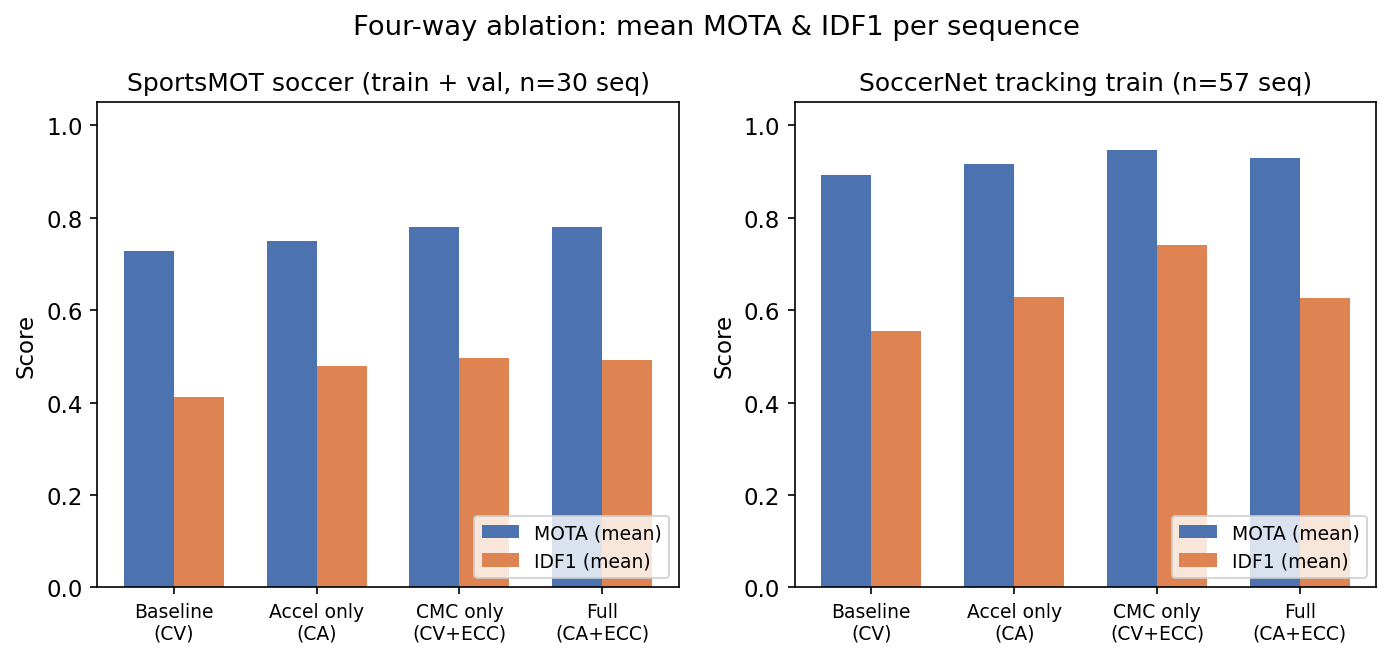
\includegraphics[width=\linewidth]{fig1_ablation_mota_idf1.png}
  \caption{\textbf{Four-way ablation (tracking).}
  Mean MOTA and IDF1 per sequence on SportsMOT soccer (train+val, 30~seq.;
  \emph{left}) and SoccerNet-Tracking train (57~seq.; \emph{right}).
  Error bars show 95\% confidence intervals over sequences.
  ECC improves both metrics on both datasets.
  \textbf{Full} matches \textbf{CMC-only} on SportsMOT but underperforms
  it on SoccerNet train under shared hyperparameters.}
  \label{fig:ablation_tracking}
\end{figure}

\begin{figure}[t]
  \centering
  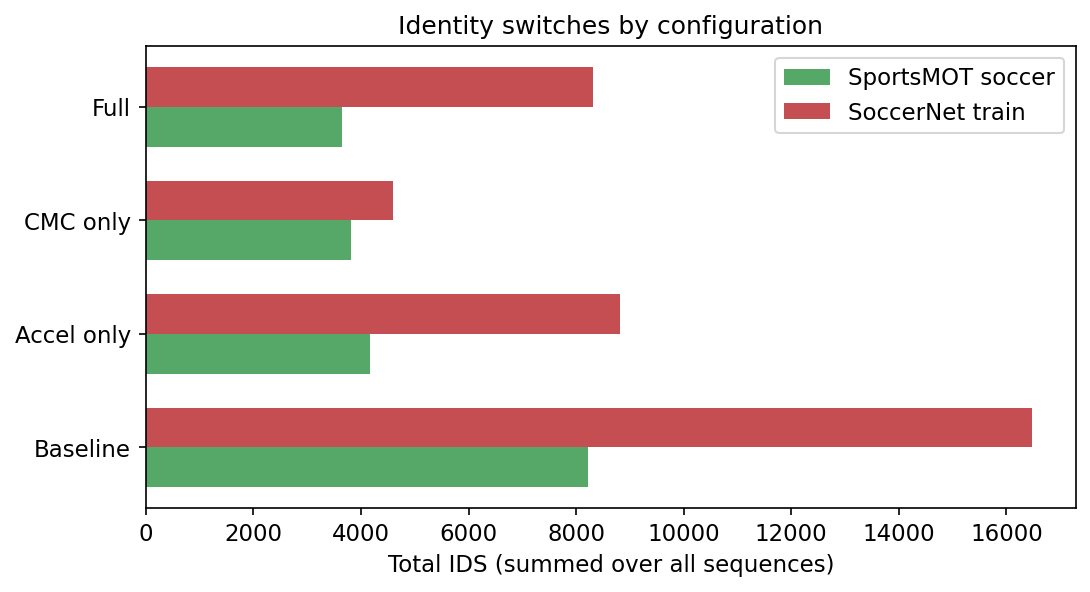
\includegraphics[width=0.92\linewidth]{fig2_ablation_ids_totals.png}
  \caption{\textbf{Identity switches by configuration.}
  Total IDS summed over all sequences (lower is better).
  SportsMOT (\emph{green}) benefits monotonically through \textbf{Full}.
  SoccerNet train (\emph{red}) is best at \textbf{CMC-only};
  \textbf{Full} increases IDS, consistent with lower IDF1 in
  Figure~\ref{fig:ablation_tracking}.}
  \label{fig:ablation_ids}
\end{figure}

\begin{figure}[t]
  \centering
  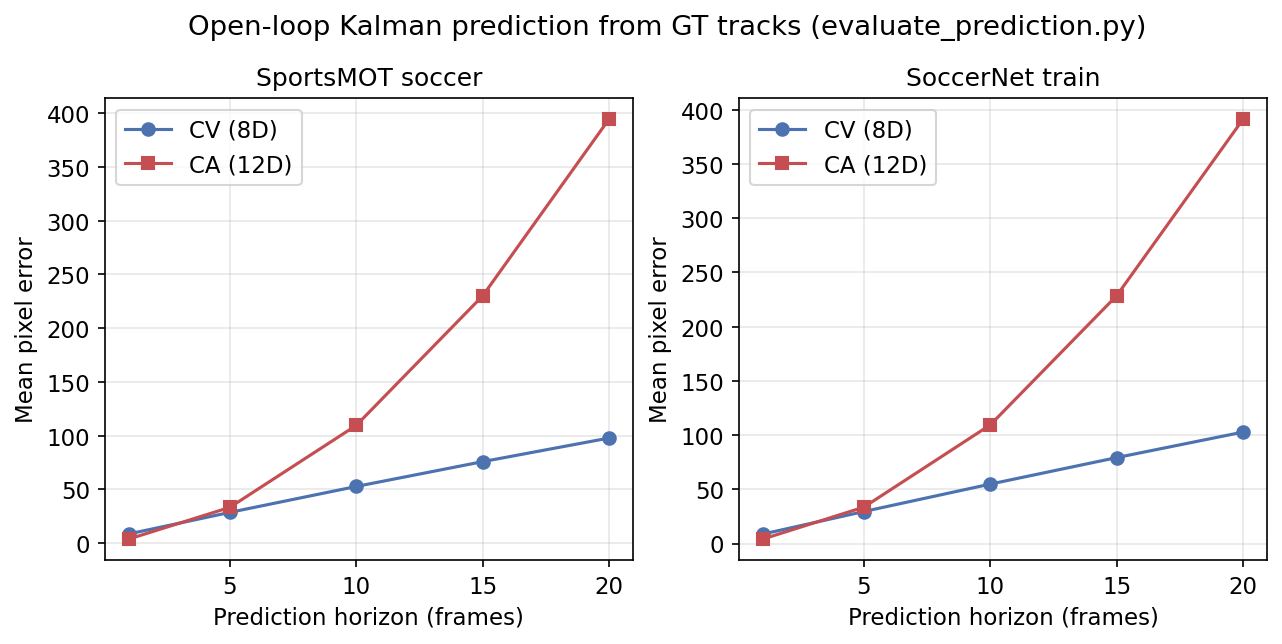
\includegraphics[width=\linewidth]{fig3_prediction_horizon.png}
  \caption{\textbf{Open-loop Kalman prediction error vs.\ horizon.}
  Mean pixel error for CV (8D) vs.\ CA (12D) filters fit to GT tracks on
  SportsMOT soccer (\emph{left}) and SoccerNet train (\emph{right}).
  CA is better at horizon~1 but degrades faster without measurements;
  long-horizon curves should not be equated with tracker association
  performance.}
  \label{fig:prediction_horizon}
\end{figure}

\begin{figure}[t]
  \centering
  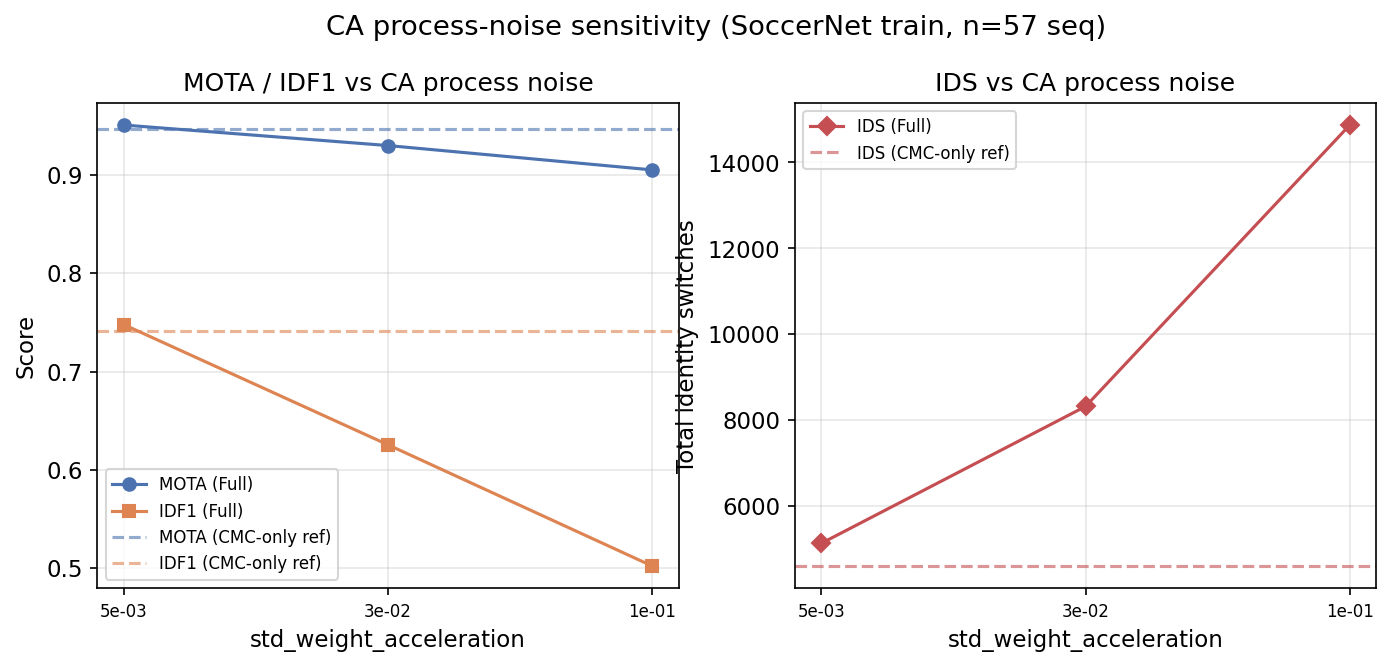
\includegraphics[width=\linewidth]{fig4_ca_sensitivity.png}
  \caption{\textbf{CA process-noise sensitivity (SoccerNet train).}
  MOTA/IDF1 (\emph{left}) and total IDS (\emph{right}) for the Full
  configuration as a function of $\sigma_\mathrm{acc}$. Dashed lines show
  CMC-only reference values. At $\sigma_\mathrm{acc} = 5 \times 10^{-3}$,
  Full matches CMC-only on both metrics; performance degrades monotonically
  with increasing noise, confirming that the main-ablation regression is a
  tuning artifact.}
  \label{fig:ca_sensitivity}
\end{figure}

\begin{figure}[t]
  \centering
  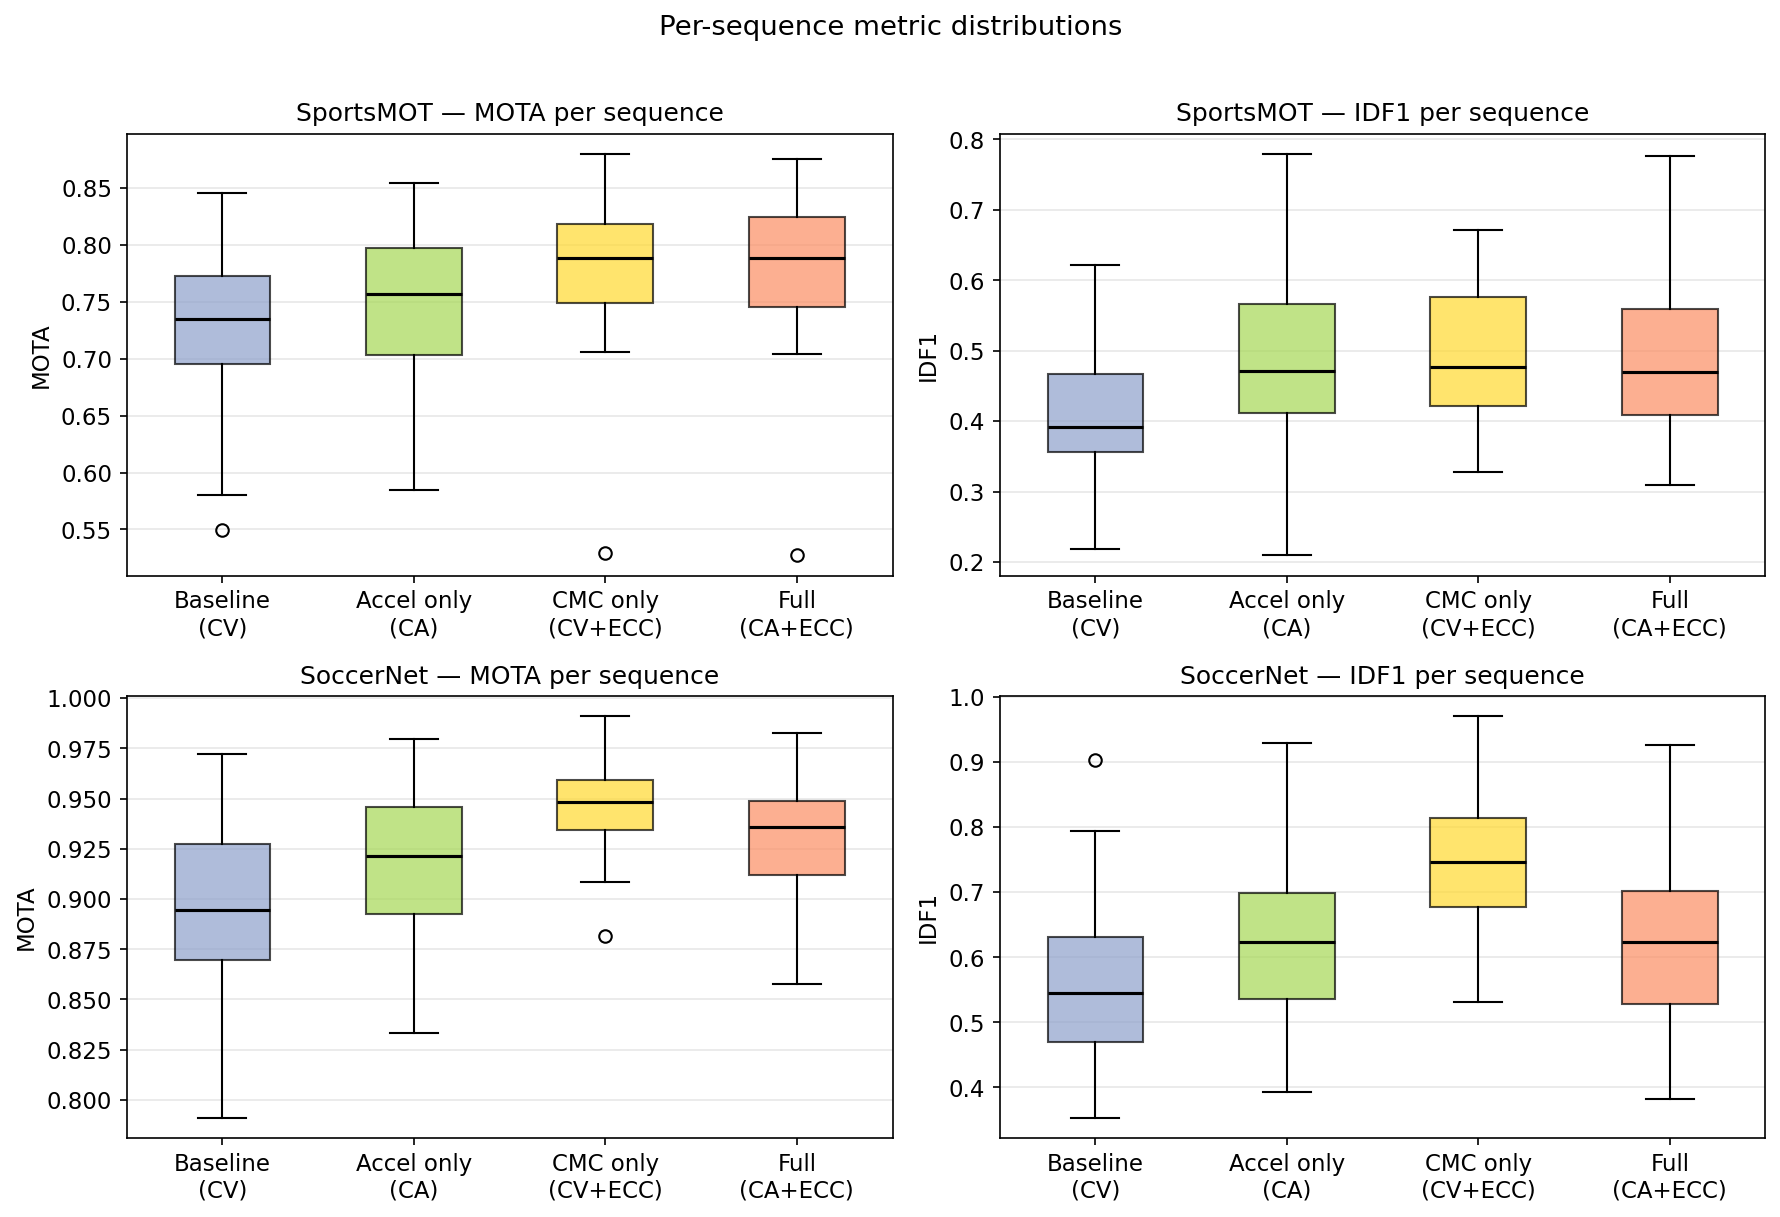
\includegraphics[width=\linewidth]{fig5_per_sequence_boxplots.png}
  \caption{\textbf{Per-sequence metric distributions.}
  Box plots of MOTA (\emph{left}) and IDF1 (\emph{right}) for each
  configuration on SportsMOT (top) and SoccerNet (bottom). On SoccerNet,
  the IDF1 distributions for CMC-only and Full show minimal overlap,
  confirming that the regression is systematic rather than driven by
  outlier sequences.}
  \label{fig:per_sequence_boxplots}
\end{figure}


% =============================================================================
% Tables
% =============================================================================

\begin{table}[t]
  \centering
  \small
  \begin{tabular}{lcccccc}
    \toprule
    & \multicolumn{3}{c}{SportsMOT ($n{=}30$)}
    & \multicolumn{3}{c}{SoccerNet ($n{=}57$)} \\
    \cmidrule(lr){2-4} \cmidrule(lr){5-7}
    Config
    & MOTA$\uparrow$ & IDF1$\uparrow$ & IDS$\downarrow$
    & MOTA$\uparrow$ & IDF1$\uparrow$ & IDS$\downarrow$ \\
    \midrule
    Baseline      & 0.729 & 0.412 & 8228  & 0.893 & 0.556 & 16469 \\
    Accel-only    & 0.749 & 0.480 & 4167  & 0.917 & 0.629 & 8814  \\
    CMC-only      & \textbf{0.781} & \textbf{0.497} & 3808
                  & \textbf{0.947} & \textbf{0.741} & \textbf{4602} \\
    Full          & 0.780 & 0.491 & \textbf{3639}
                  & 0.930 & 0.626 & 8319 \\
    \bottomrule
  \end{tabular}
  \caption{Mean MOTA and IDF1 per sequence; IDS summed over all sequences.
  Best values per dataset in bold. On SportsMOT, Full achieves the lowest
  IDS while matching CMC-only on MOTA/IDF1. On SoccerNet, CMC-only
  dominates across all three metrics.}
  \label{tab:ablation}
\end{table}

\begin{table}[t]
  \centering
  \small
  \begin{tabular}{lcccc}
    \toprule
    & \multicolumn{2}{c}{SportsMOT ($n{=}30$)}
    & \multicolumn{2}{c}{SoccerNet ($n{=}57$)} \\
    \cmidrule(lr){2-3} \cmidrule(lr){4-5}
    Comparison & MOTA & IDF1 & MOTA & IDF1 \\
    \midrule
    Baseline vs.\ Accel-only
      & .001\rlap{$^{**}$}  & $<$.001\rlap{$^{***}$}
      & $<$.001\rlap{$^{***}$} & $<$.001\rlap{$^{***}$} \\
    Baseline vs.\ CMC-only
      & $<$.001\rlap{$^{***}$} & $<$.001\rlap{$^{***}$}
      & $<$.001\rlap{$^{***}$} & $<$.001\rlap{$^{***}$} \\
    Baseline vs.\ Full
      & $<$.001\rlap{$^{***}$} & $<$.001\rlap{$^{***}$}
      & $<$.001\rlap{$^{***}$} & $<$.001\rlap{$^{***}$} \\
    Accel-only vs.\ CMC-only
      & $<$.001\rlap{$^{***}$} & .146\phantom{$^{***}$}
      & $<$.001\rlap{$^{***}$} & $<$.001\rlap{$^{***}$} \\
    Accel-only vs.\ Full
      & $<$.001\rlap{$^{***}$} & .855\phantom{$^{***}$}
      & $<$.001\rlap{$^{***}$} & .015\rlap{$^{*}$}\phantom{$^{**}$} \\
    CMC-only vs.\ Full
      & .253\phantom{$^{***}$} & .029\phantom{$^{***}$}
      & $<$.001\rlap{$^{***}$} & $<$.001\rlap{$^{***}$} \\
    \bottomrule
  \end{tabular}
  \caption{Paired Wilcoxon signed-rank $p$-values (two-sided, uncorrected).
  $^{*}\!p<.05$,\; $^{**}\!p<.01$,\; $^{***}\!p<.001$.
  All configurations differ significantly from Baseline.
  CMC-only vs.\ Full is not significant on SportsMOT (MOTA $p{=}.25$,
  IDF1 $p{=}.029$ --- would not survive Bonferroni correction for 6
  comparisons) but highly significant on SoccerNet ($p < 10^{-9}$).}
  \label{tab:significance}
\end{table}

\begin{table}[t]
  \centering
  \small
  \begin{tabular}{lccccc}
    \toprule
    & \multicolumn{5}{c}{Identity switches by regime} \\
    \cmidrule(lr){2-6}
    Config & Accel & Pan & Both & Neither & Total \\
    \midrule
    \multicolumn{6}{l}{\emph{SportsMOT (train+val, 30 seq.)}} \\
    Baseline      & 3230 & ---  & ---  & 4998 & 8228 \\
    Accel-only    & 1752 & ---  & ---  & 2415 & 4167 \\
    CMC-only      &  423 &  893 &  826 & 1666 & 3808 \\
    Full          &  356 &  895 &  840 & 1548 & 3639 \\
    \midrule
    \multicolumn{6}{l}{\emph{SoccerNet train (57 seq.)}} \\
    Baseline      & 14054 & --- & ---  & 2415 & 16469 \\
    Accel-only    &  7479 & --- & ---  & 1335 &  8814 \\
    CMC-only      &   607 & 557 & 2838 &  600 &  4602 \\
    Full          &   716 & 435 & 6631 &  537 &  8319 \\
    \bottomrule
  \end{tabular}
  \caption{Identity switches broken down by frame regime. ``---'' indicates
  that pan detection is unavailable without CMC enabled. On SoccerNet, Full
  produces 6{,}631 switches during frames with simultaneous acceleration and
  pan events, vs.\ 2{,}838 for CMC-only---the primary source of the Full
  regression.}
  \label{tab:regime}
\end{table}
 set graphics path,
% e.g. from repository root:
%   \graphicspath{{results/analysis/figures/}}
%
% Or copy the PNGs into your paper's ./figures/ and use that folder instead.
% =============================================================================

\section{Experiments}
\label{sec:experiments}

We evaluate through three complementary protocols: a $2 \times 2$ factorial
ablation of tracker configurations, an open-loop Kalman prediction test on
ground-truth tracks, and a per-frame regime analysis that classifies
identity switches by whether they occur during acceleration events, camera
pans, or both.

A $2 \times 2$ factorial design crossing two binary factors, constant-acceleration
Kalman filter (CA) and ECC camera-motion compensation (CMC), yields four
tracker configurations:

\begin{itemize}
    \item \textbf{Baseline} (constant-velocity KF, no CMC),
    \item \textbf{Accel-only} (constant-acceleration KF, no CMC),
    \item \textbf{CMC-only} (constant-velocity KF with ECC), and
    \item \textbf{Full} (constant-acceleration KF with ECC).
\end{itemize}
All four share the same offline detections, the same Re-ID
configuration, and the same association hyperparameters; only the motion
model and compensation module differ. This ensures that any difference in
tracking metrics is attributable to our modifications rather than to
confounding factors.

We measure the open-loop Kalman prediction quality by fitting both
constant-velocity (8D) and constant-acceleration (12D) filters to
ground-truth bounding-box trajectories. At regular intervals (every 5
frames, after at least 10 frames of history), we predict forward
\emph{without any measurement updates} and record the Euclidean distance
between the predicted and true bounding-box centers at horizons
$h \in \{1, 5, 10, 15, 20\}$ frames. This test isolates the motion model's
extrapolation quality from the association step.

We report standard MOTChallenge metrics computed via the
\texttt{py-motmetrics} library with an IoU matching threshold of 0.5. Our
primary metric is IDF1, which directly measures identity preservation over
time and is the most relevant quantity for sports analytics where correct
player identity matters more than detection completeness. We report MOTA for
comparability with prior work, alongside raw identity-switch counts (IDS)
summed over all sequences.

To test whether the two fixes target separable failure modes, we classify
each frame into one of four regimes based on ground-truth trajectories and
ECC warp estimates. A frame is flagged as an \emph{acceleration event} if
any tracked player's velocity changes by more than 15~px/frame$^2$ within a
$\pm 3$-frame window. A frame is flagged as a \emph{camera-pan event} if the
ECC-estimated affine translation magnitude exceeds 5~px. Frames can be
flagged as both, either, or neither. We then count identity switches
occurring within each regime. If the constant-acceleration filter primarily
reduces switches during acceleration events while CMC primarily reduces
switches during pan events, the two modules address orthogonal failure
modes.


Person detections are generated offline using
YOLOv8x~\cite{jocher2023yolov8} pretrained on COCO. We run inference at
1280-pixel resolution with a confidence threshold of~0.3, retaining only
COCO class~0 (person). The resulting bounding boxes are written in
MOTChallenge text format. At tracking time, an additional confidence filter
at~0.5 and non-maximum suppression are applied. Crucially, all four
DeepSORT ablation variants consume the same detection files, so differences
in MOTA, IDF1, and IDS are attributable solely to the tracker.

We deliberately disable the Re-ID appearance branch by using a dummy
feature extractor that returns zero vectors for all detections. DeepSORT's
cascade matching still runs---confirmed tracks are prioritized by recency,
and an IoU-based fallback handles unmatched detections---but the cosine
distance between any two features is constant, so association depends
entirely on Kalman-predicted position and Mahalanobis/IoU gating. This
design choice isolates the effect of our motion-model modifications: with
appearance features active, improvements from the Kalman filter or CMC could
be masked by the Re-ID network independently correcting association errors.
We note that this makes the ablation a harder test of the motion model and
that our reported metrics are conservative relative to what a
soccer-fine-tuned Re-ID network would achieve.

All DeepSORT variants share the same association and lifecycle parameters:
cosine distance threshold~0.3, IoU fallback gate~0.7, appearance gallery
budget of~100 per track, $\text{max\_age} = 30$ frames before track
deletion, and $n_\text{init} = 3$ hits before track confirmation. For the
constant-velocity filter, process-noise weights are
$\sigma_\text{pos} = 10^{-2}$ and $\sigma_\text{vel} = 10^{-5}$ (scaled by
bounding-box height). The constant-acceleration filter uses the same
position and velocity noise, with an acceleration process-noise weight of
$\sigma_\text{acc} = 2.5 \times 10^{-2}$. This deliberately high
acceleration noise is a key tuning decision: it allows the filter to absorb
sudden directional changes---a player cutting left after sprinting
right---without remaining overconfident in a now-stale acceleration
estimate.

Camera-motion compensation uses OpenCV's Enhanced Correlation Coefficient
(ECC) algorithm in affine mode (6~DOF: translation, rotation, scale, shear).
We set the maximum iteration count to~50 with a convergence threshold of
$10^{-3}$. Frames are downscaled by a factor of~2 and Gaussian-blurred with
$\sigma = 1.5$ before ECC estimation, balancing speed against registration
robustness. When ECC fails to converge (e.g., during shot changes), the
identity warp is applied, resulting in no compensation for that frame.


% ─────────────────────────────────────────────────────────────────────────────
\subsection{Results}
\label{sec:results}
% ─────────────────────────────────────────────────────────────────────────────


We evaluate four tracker variants as described in
Section~\ref{sec:experiments}. We report MOTA and IDF1 averaged over
sequences and IDS summed over sequences (fewer identity switches is better).
On the SportsMOT soccer subset we pool the train and validation splits
(30~sequences, 53{,}913~frames); on
SoccerNet-Tracking~\cite{cioppa2022soccernettracking} we evaluate the train
split (57~sequences, 42{,}750~frames). Pooling train and validation on
SportsMOT gives a larger and more stable per-variant comparison on a fixed
set of sequences; readers seeking benchmark-aligned headline numbers may
prefer validation- or test-only evaluation.

SportsMOT sequences ship with per-frame detections; where missing, we
generate person-class boxes with YOLOv8x ($\mathrm{conf} > 0.3$).
SoccerNet-Tracking provides annotation-derived detections with the dataset.
Because detector quality and recall differ, cross-dataset metric comparisons
reflect joint tracker\,+\,detector performance and should be interpreted
accordingly. All within-dataset ablation comparisons use identical
detections and thus isolate tracker contributions.


Table~\ref{tab:ablation} and Figure~\ref{fig:ablation_tracking} show mean
MOTA and IDF1 per sequence for each configuration, with error bars
indicating 95\% confidence intervals computed over sequences.
On \textbf{SportsMOT}, enabling camera compensation
yields the largest gains: CMC-only and Full both reach MOTA~$\approx 0.78$,
clearly above Baseline ($\approx 0.73$). IDF1 follows the same trend, with
CMC-only slightly strongest among the ECC variants. On
\textbf{SoccerNet train}, CMC-only is best overall (MOTA~$\approx 0.95$,
IDF1~$\approx 0.74$). Adding acceleration on top of ECC (Full) does not
improve headline metrics on this split; MOTA and especially IDF1 drop
relative to CMC-only, while Accel-only remains a substantial improvement
over Baseline.

Figure~\ref{fig:ablation_ids} reports the same trend through identity
switches. On SportsMOT, IDS decreases monotonically from Baseline through
Full, confirming that the two fixes are complementary on this dataset. On
SoccerNet, IDS is lowest for CMC-only and rises again for Full.

\paragraph{Statistical significance.}
Paired Wilcoxon signed-rank tests (Table~\ref{tab:significance}) confirm
that every configuration differs significantly from Baseline on both
datasets ($p < .002$, uncorrected). On SportsMOT, the difference between
CMC-only and Full is \emph{not} significant for MOTA ($p = .25$); the
nominal $p = .029$ for IDF1 would not survive Bonferroni correction for the
six pairwise comparisons ($\alpha_\text{adj} = .05/6 \approx .008$),
consistent with the overlapping confidence intervals in
Figure~\ref{fig:ablation_tracking}. On SoccerNet, the CMC-only vs.\ Full
gap is highly significant for both metrics ($p < 10^{-9}$, well below any
corrected threshold), confirming that the regression is systematic rather
than driven by a few outlier sequences. Per-sequence distributions
(Figure~\ref{fig:per_sequence_boxplots}) corroborate this: the SoccerNet
IDF1 boxes for CMC-only and Full show minimal overlap.

Together, Figures~\ref{fig:ablation_tracking}--\ref{fig:ablation_ids}
and Table~\ref{tab:significance} indicate that \textbf{ECC camera-motion
compensation is the dominant improvement under shared hyperparameters}.
Combining the constant-acceleration KF with ECC improves identity stability
on SportsMOT but hurts it on SoccerNet train in our configuration,
suggesting that the acceleration noise parameters require dataset-dependent
tuning rather than a universally optimal ``full'' stack.

\paragraph{Regime analysis.}
To diagnose where the Full configuration fails, we classify each identity
switch by what was happening in that frame (Table~\ref{tab:regime}). On
SportsMOT, moving from Baseline to Accel-only reduces acceleration-regime
IDS from 3{,}230 to 1{,}752 (46\% reduction). CMC-only reduces it further
to~423 (87\% vs.\ Baseline). Full provides marginal additional reduction
(356) with similar pan-regime counts, consistent with the complementary
behavior observed above.

On SoccerNet, the pattern is more revealing. Baseline produces 14{,}054
acceleration-regime IDS; Accel-only cuts this to 7{,}479 (47\%). CMC-only
reduces acceleration-regime IDS to 607 but produces 2{,}838 switches in
frames with simultaneous acceleration and pan events. Full \emph{increases}
this both-regime count to 6{,}631---nearly all of the IDS regression
originates in these complex frames where both player acceleration and camera
motion occur simultaneously.

The divergent behavior between datasets has a plausible explanation.
SportsMOT sequences are short clips (typically under 2{,}000~frames) filmed
from overhead cameras with moderate panning, where bursty player motion is
the primary source of prediction error. SoccerNet sequences are longer
broadcast footage with aggressive panning and zooming, where camera
ego-motion dominates. In the SoccerNet regime, the additional acceleration
states in the 12D filter introduce extra degrees of freedom that, without
dataset-specific noise tuning, can amplify drift during extended occlusions.
This is consistent with the well-known bias--variance tradeoff in Kalman
filter design: a higher-dimensional state improves fit to complex dynamics
but increases estimation noise when measurements are sparse.

\paragraph{Process-noise sensitivity.}
To investigate whether the Full-configuration regression on SoccerNet is
structural or parametric, we sweep the CA process-noise scale
$\sigma_\mathrm{acc} \in \{5 \times 10^{-3},\; 2.5 \times 10^{-2},\;
10^{-1}\}$ with ECC enabled (Figure~\ref{fig:ca_sensitivity}).
At the lowest noise value ($\sigma_\mathrm{acc} = 5 \times 10^{-3}$),
the Full configuration achieves MOTA\,=\,0.951 and IDF1\,=\,0.748,
\emph{matching or slightly exceeding} the CMC-only reference
(MOTA\,=\,0.947, IDF1\,=\,0.741). Performance degrades monotonically
as noise increases: the default value used in the main ablation
($\sigma_\mathrm{acc} = 2.5 \times 10^{-2}$) already falls well below
CMC-only, and at $10^{-1}$ the tracker loses over 14{,}800 identities.
This confirms that the regression is a tuning artifact rather than a
fundamental incompatibility between CA dynamics and ECC-stabilized
coordinates: with conservative acceleration noise, the 12D filter
neither helps nor hurts on SoccerNet, while retaining its benefits on
SportsMOT.

\subsection{Kalman prediction analysis}

Figure~\ref{fig:prediction_horizon} compares the open-loop center error of
the constant-velocity (8D) and constant-acceleration (12D) Kalman filters
fit to ground-truth tracks at prediction horizons
$h \in \{1, 5, 10, 15, 20\}$ frames. On both datasets, the
constant-acceleration filter achieves \textbf{lower error at $h = 1$},
confirming that one-step prediction benefits from modeling acceleration.
However, error grows faster for the CA filter at longer horizons, surpassing
the CV filter by $h \geq 5$.

This behavior is expected when forecasting without measurements: the extra
acceleration state helps capture immediate dynamics but amplifies drift when
no corrective observations are available. We emphasize that
Figure~\ref{fig:prediction_horizon} is \emph{not} contradictory with the
tracker metrics. In the actual tracking loop, measurement updates arrive
every frame, so the Kalman filter rarely operates in open-loop mode for more
than a few frames (except during occlusions). The one-step advantage of the
CA filter is what matters for frame-to-frame association, while the
long-horizon degradation explains why the CA filter can hurt performance
during extended occlusions---precisely the regime where SoccerNet's longer,
more complex sequences expose the weakness.

\subsection{Limitations}

Several limitations apply to our evaluation. First, SportsMOT relies on
generated detections where sequences were missing pre-computed detection
files, while SoccerNet uses its dataset-provided detections. This means the
detection quality is not perfectly controlled across datasets, although it
is controlled within each dataset across all four ablation variants.

Second, we do not report SoccerNet test or challenge splits, as these
require submission to the official evaluation server. Our pooled train+val
evaluation on SportsMOT is kept for stable per-variant comparison rather
than benchmark headline numbers.

Third, our ablation deliberately disables the Re-ID appearance branch to
isolate motion-model effects. Our reported metrics represent a lower bound
on what our modifications would achieve when combined with a
soccer-fine-tuned Re-ID network. Integrating domain-specific appearance
features is a natural extension of this work.

Fourth, all four variants share a single set of hyperparameters. The
SoccerNet results suggest that the constant-acceleration filter's
process-noise covariance would benefit from per-dataset or per-sequence
tuning. Adaptive noise estimation---for example, using innovation-based
scaling~\cite{cao2023observationcentricsortrethinkingsort}---is another
promising direction.


% =============================================================================
% Figures
% =============================================================================

\begin{figure}[t]
  \centering
  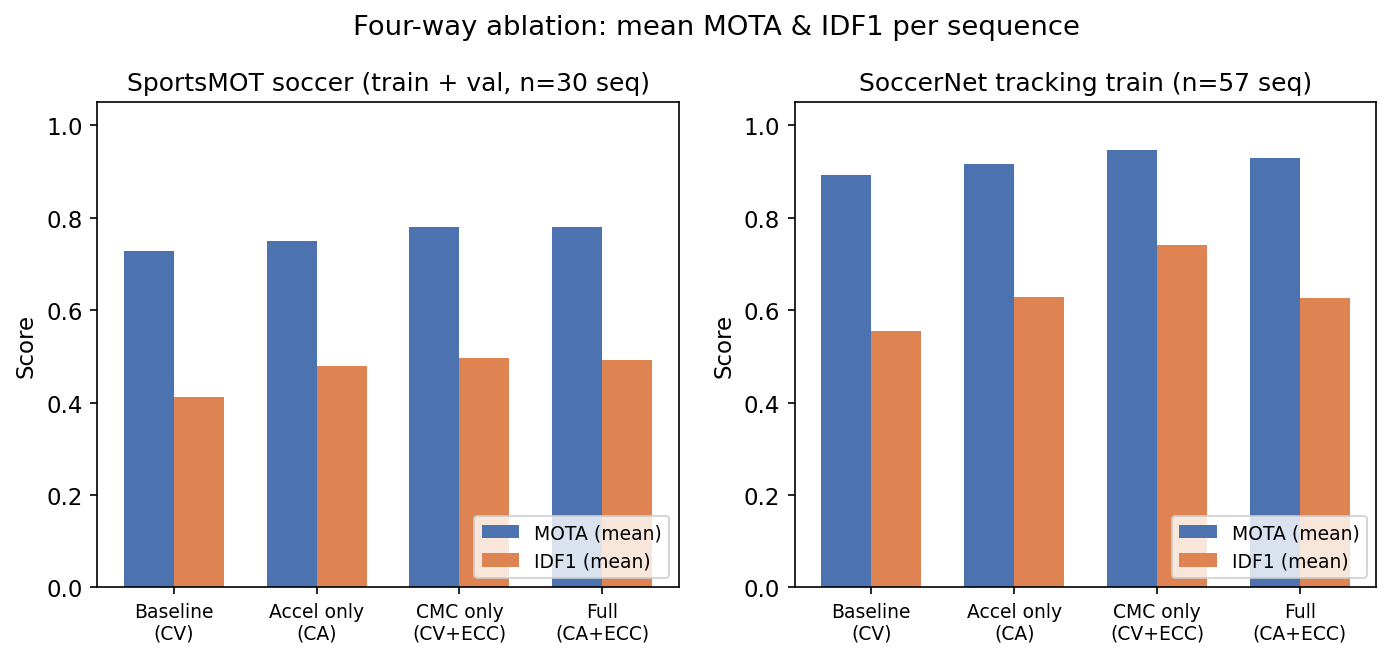
\includegraphics[width=\linewidth]{fig1_ablation_mota_idf1.png}
  \caption{\textbf{Four-way ablation (tracking).}
  Mean MOTA and IDF1 per sequence on SportsMOT soccer (train+val, 30~seq.;
  \emph{left}) and SoccerNet-Tracking train (57~seq.; \emph{right}).
  Error bars show 95\% confidence intervals over sequences.
  ECC improves both metrics on both datasets.
  \textbf{Full} matches \textbf{CMC-only} on SportsMOT but underperforms
  it on SoccerNet train under shared hyperparameters.}
  \label{fig:ablation_tracking}
\end{figure}

\begin{figure}[t]
  \centering
  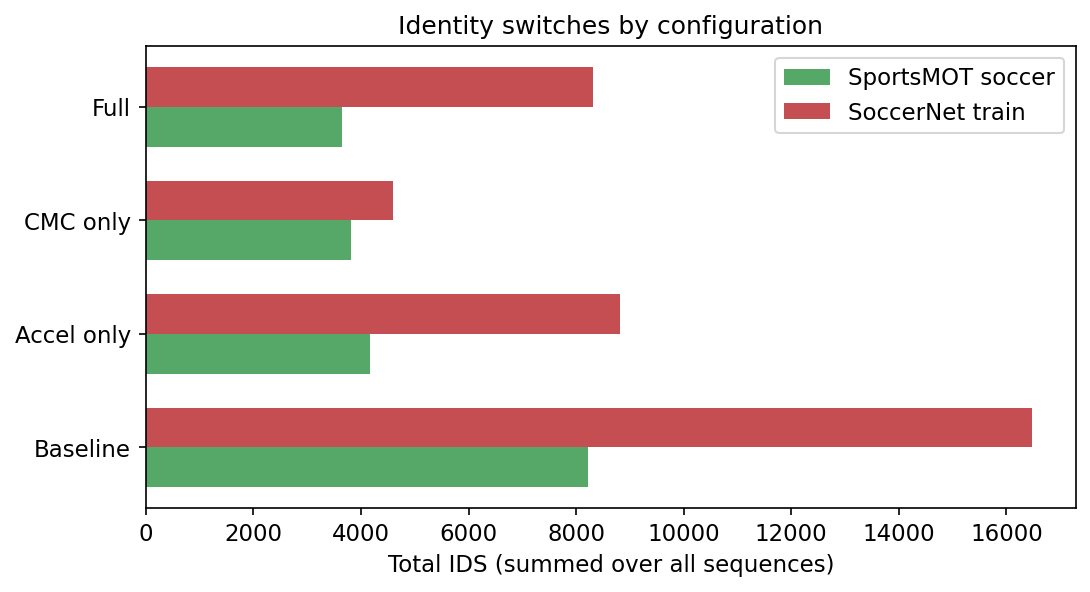
\includegraphics[width=0.92\linewidth]{fig2_ablation_ids_totals.png}
  \caption{\textbf{Identity switches by configuration.}
  Total IDS summed over all sequences (lower is better).
  SportsMOT (\emph{green}) benefits monotonically through \textbf{Full}.
  SoccerNet train (\emph{red}) is best at \textbf{CMC-only};
  \textbf{Full} increases IDS, consistent with lower IDF1 in
  Figure~\ref{fig:ablation_tracking}.}
  \label{fig:ablation_ids}
\end{figure}

\begin{figure}[t]
  \centering
  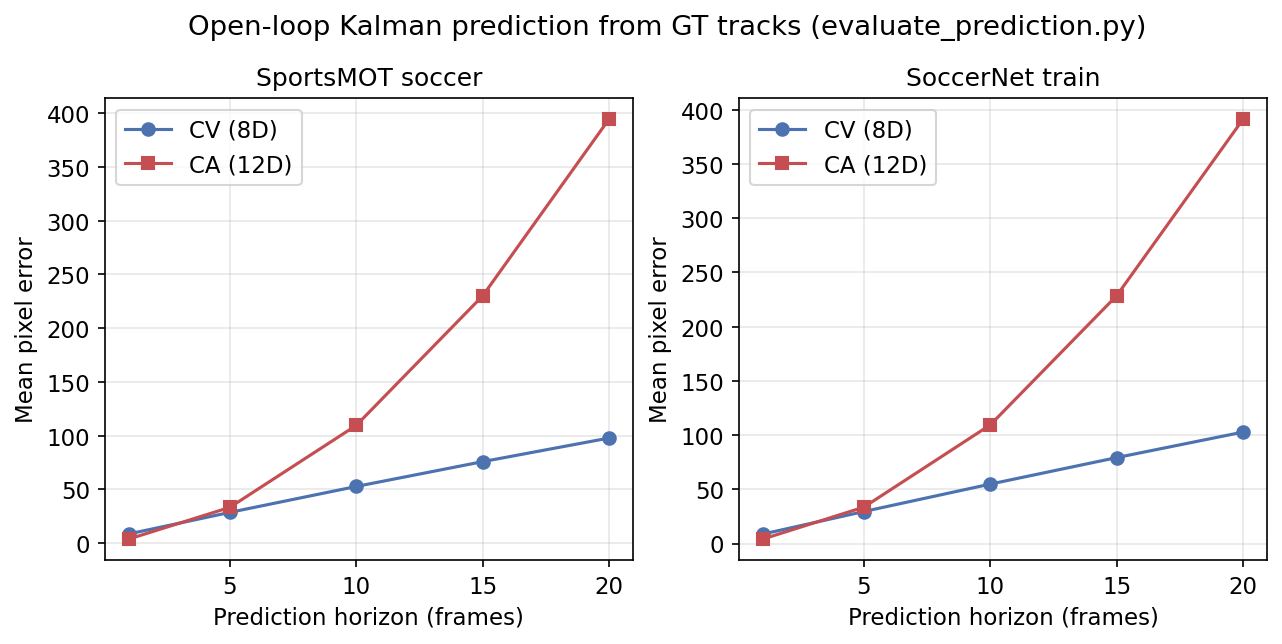
\includegraphics[width=\linewidth]{fig3_prediction_horizon.png}
  \caption{\textbf{Open-loop Kalman prediction error vs.\ horizon.}
  Mean pixel error for CV (8D) vs.\ CA (12D) filters fit to GT tracks on
  SportsMOT soccer (\emph{left}) and SoccerNet train (\emph{right}).
  CA is better at horizon~1 but degrades faster without measurements;
  long-horizon curves should not be equated with tracker association
  performance.}
  \label{fig:prediction_horizon}
\end{figure}

\begin{figure}[t]
  \centering
  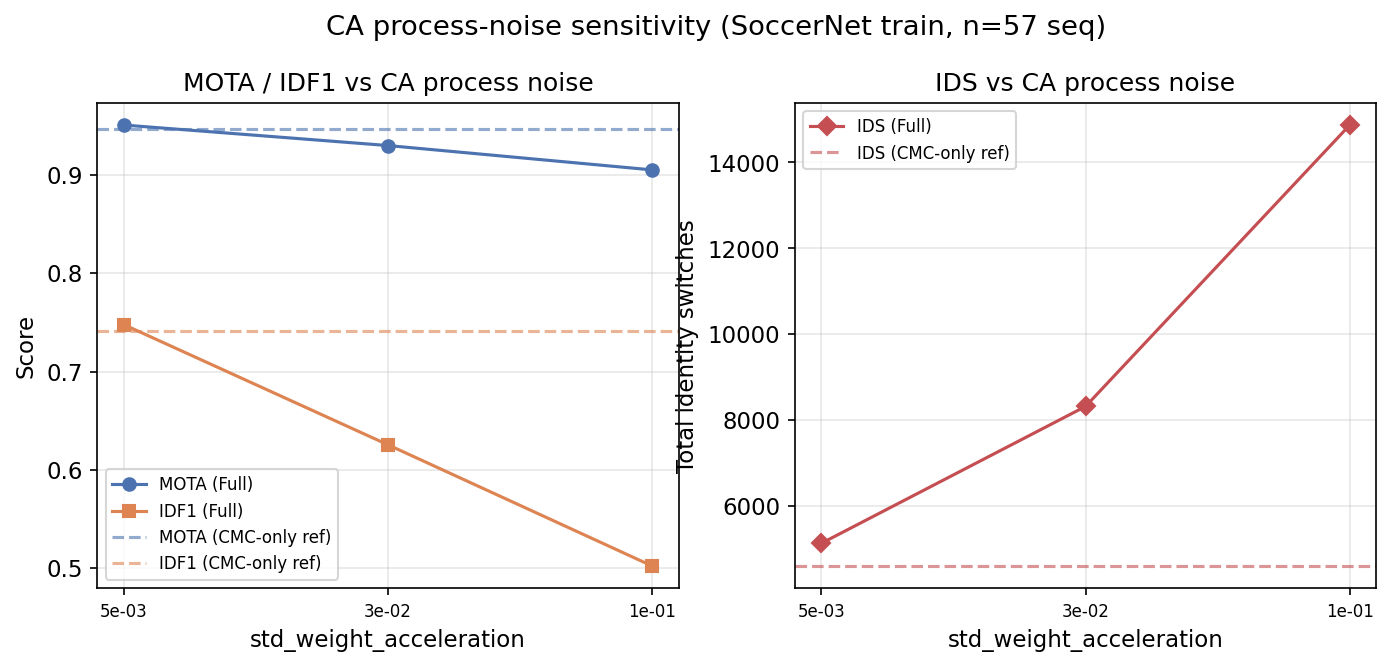
\includegraphics[width=\linewidth]{fig4_ca_sensitivity.png}
  \caption{\textbf{CA process-noise sensitivity (SoccerNet train).}
  MOTA/IDF1 (\emph{left}) and total IDS (\emph{right}) for the Full
  configuration as a function of $\sigma_\mathrm{acc}$. Dashed lines show
  CMC-only reference values. At $\sigma_\mathrm{acc} = 5 \times 10^{-3}$,
  Full matches CMC-only on both metrics; performance degrades monotonically
  with increasing noise, confirming that the main-ablation regression is a
  tuning artifact.}
  \label{fig:ca_sensitivity}
\end{figure}

\begin{figure}[t]
  \centering
  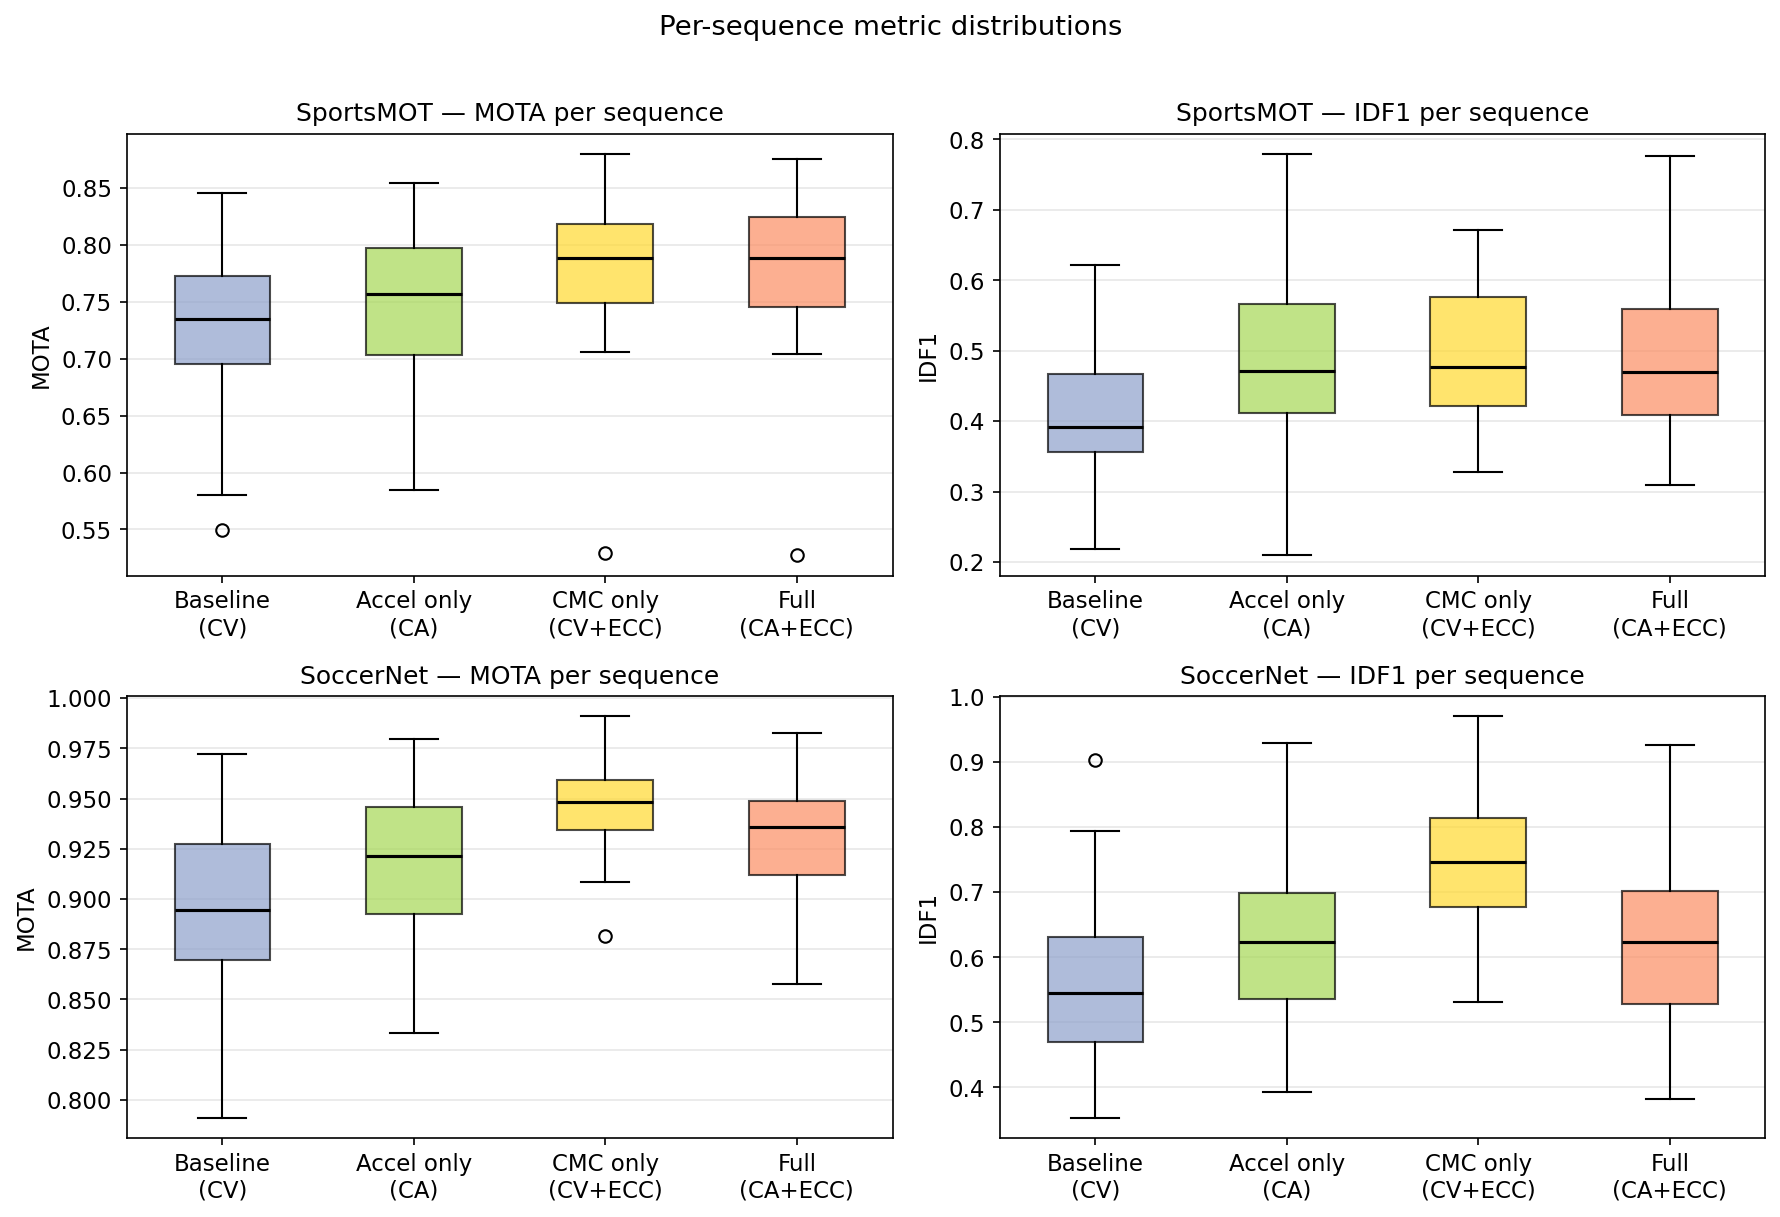
\includegraphics[width=\linewidth]{fig5_per_sequence_boxplots.png}
  \caption{\textbf{Per-sequence metric distributions.}
  Box plots of MOTA (\emph{left}) and IDF1 (\emph{right}) for each
  configuration on SportsMOT (top) and SoccerNet (bottom). On SoccerNet,
  the IDF1 distributions for CMC-only and Full show minimal overlap,
  confirming that the regression is systematic rather than driven by
  outlier sequences.}
  \label{fig:per_sequence_boxplots}
\end{figure}


% =============================================================================
% Tables
% =============================================================================

\begin{table}[t]
  \centering
  \small
  \begin{tabular}{lcccccc}
    \toprule
    & \multicolumn{3}{c}{SportsMOT ($n{=}30$)}
    & \multicolumn{3}{c}{SoccerNet ($n{=}57$)} \\
    \cmidrule(lr){2-4} \cmidrule(lr){5-7}
    Config
    & MOTA$\uparrow$ & IDF1$\uparrow$ & IDS$\downarrow$
    & MOTA$\uparrow$ & IDF1$\uparrow$ & IDS$\downarrow$ \\
    \midrule
    Baseline      & 0.729 & 0.412 & 8228  & 0.893 & 0.556 & 16469 \\
    Accel-only    & 0.749 & 0.480 & 4167  & 0.917 & 0.629 & 8814  \\
    CMC-only      & \textbf{0.781} & \textbf{0.497} & 3808
                  & \textbf{0.947} & \textbf{0.741} & \textbf{4602} \\
    Full          & 0.780 & 0.491 & \textbf{3639}
                  & 0.930 & 0.626 & 8319 \\
    \bottomrule
  \end{tabular}
  \caption{Mean MOTA and IDF1 per sequence; IDS summed over all sequences.
  Best values per dataset in bold. On SportsMOT, Full achieves the lowest
  IDS while matching CMC-only on MOTA/IDF1. On SoccerNet, CMC-only
  dominates across all three metrics.}
  \label{tab:ablation}
\end{table}

\begin{table}[t]
  \centering
  \small
  \begin{tabular}{lcccc}
    \toprule
    & \multicolumn{2}{c}{SportsMOT ($n{=}30$)}
    & \multicolumn{2}{c}{SoccerNet ($n{=}57$)} \\
    \cmidrule(lr){2-3} \cmidrule(lr){4-5}
    Comparison & MOTA & IDF1 & MOTA & IDF1 \\
    \midrule
    Baseline vs.\ Accel-only
      & .001\rlap{$^{**}$}  & $<$.001\rlap{$^{***}$}
      & $<$.001\rlap{$^{***}$} & $<$.001\rlap{$^{***}$} \\
    Baseline vs.\ CMC-only
      & $<$.001\rlap{$^{***}$} & $<$.001\rlap{$^{***}$}
      & $<$.001\rlap{$^{***}$} & $<$.001\rlap{$^{***}$} \\
    Baseline vs.\ Full
      & $<$.001\rlap{$^{***}$} & $<$.001\rlap{$^{***}$}
      & $<$.001\rlap{$^{***}$} & $<$.001\rlap{$^{***}$} \\
    Accel-only vs.\ CMC-only
      & $<$.001\rlap{$^{***}$} & .146\phantom{$^{***}$}
      & $<$.001\rlap{$^{***}$} & $<$.001\rlap{$^{***}$} \\
    Accel-only vs.\ Full
      & $<$.001\rlap{$^{***}$} & .855\phantom{$^{***}$}
      & $<$.001\rlap{$^{***}$} & .015\rlap{$^{*}$}\phantom{$^{**}$} \\
    CMC-only vs.\ Full
      & .253\phantom{$^{***}$} & .029\phantom{$^{***}$}
      & $<$.001\rlap{$^{***}$} & $<$.001\rlap{$^{***}$} \\
    \bottomrule
  \end{tabular}
  \caption{Paired Wilcoxon signed-rank $p$-values (two-sided, uncorrected).
  $^{*}\!p<.05$,\; $^{**}\!p<.01$,\; $^{***}\!p<.001$.
  All configurations differ significantly from Baseline.
  CMC-only vs.\ Full is not significant on SportsMOT (MOTA $p{=}.25$,
  IDF1 $p{=}.029$ --- would not survive Bonferroni correction for 6
  comparisons) but highly significant on SoccerNet ($p < 10^{-9}$).}
  \label{tab:significance}
\end{table}

\begin{table}[t]
  \centering
  \small
  \begin{tabular}{lccccc}
    \toprule
    & \multicolumn{5}{c}{Identity switches by regime} \\
    \cmidrule(lr){2-6}
    Config & Accel & Pan & Both & Neither & Total \\
    \midrule
    \multicolumn{6}{l}{\emph{SportsMOT (train+val, 30 seq.)}} \\
    Baseline      & 3230 & ---  & ---  & 4998 & 8228 \\
    Accel-only    & 1752 & ---  & ---  & 2415 & 4167 \\
    CMC-only      &  423 &  893 &  826 & 1666 & 3808 \\
    Full          &  356 &  895 &  840 & 1548 & 3639 \\
    \midrule
    \multicolumn{6}{l}{\emph{SoccerNet train (57 seq.)}} \\
    Baseline      & 14054 & --- & ---  & 2415 & 16469 \\
    Accel-only    &  7479 & --- & ---  & 1335 &  8814 \\
    CMC-only      &   607 & 557 & 2838 &  600 &  4602 \\
    Full          &   716 & 435 & 6631 &  537 &  8319 \\
    \bottomrule
  \end{tabular}
  \caption{Identity switches broken down by frame regime. ``---'' indicates
  that pan detection is unavailable without CMC enabled. On SoccerNet, Full
  produces 6{,}631 switches during frames with simultaneous acceleration and
  pan events, vs.\ 2{,}838 for CMC-only---the primary source of the Full
  regression.}
  \label{tab:regime}
\end{table}
 set graphics path,
% e.g. from repository root:
%   \graphicspath{{results/analysis/figures/}}
%
% Or copy the PNGs into your paper's ./figures/ and use that folder instead.
% =============================================================================

\section{Experiments}
\label{sec:experiments}

We evaluate through three complementary protocols: a $2 \times 2$ factorial
ablation of tracker configurations, an open-loop Kalman prediction test on
ground-truth tracks, and a per-frame regime analysis that classifies
identity switches by whether they occur during acceleration events, camera
pans, or both.

A $2 \times 2$ factorial design crossing two binary factors, constant-acceleration
Kalman filter (CA) and ECC camera-motion compensation (CMC), yields four
tracker configurations:

\begin{itemize}
    \item \textbf{Baseline} (constant-velocity KF, no CMC),
    \item \textbf{Accel-only} (constant-acceleration KF, no CMC),
    \item \textbf{CMC-only} (constant-velocity KF with ECC), and
    \item \textbf{Full} (constant-acceleration KF with ECC).
\end{itemize}
All four share the same offline detections, the same Re-ID
configuration, and the same association hyperparameters; only the motion
model and compensation module differ. This ensures that any difference in
tracking metrics is attributable to our modifications rather than to
confounding factors.

We measure the open-loop Kalman prediction quality by fitting both
constant-velocity (8D) and constant-acceleration (12D) filters to
ground-truth bounding-box trajectories. At regular intervals (every 5
frames, after at least 10 frames of history), we predict forward
\emph{without any measurement updates} and record the Euclidean distance
between the predicted and true bounding-box centers at horizons
$h \in \{1, 5, 10, 15, 20\}$ frames. This test isolates the motion model's
extrapolation quality from the association step.

We report standard MOTChallenge metrics computed via the
\texttt{py-motmetrics} library with an IoU matching threshold of 0.5. Our
primary metric is IDF1, which directly measures identity preservation over
time and is the most relevant quantity for sports analytics where correct
player identity matters more than detection completeness. We report MOTA for
comparability with prior work, alongside raw identity-switch counts (IDS)
summed over all sequences.

To test whether the two fixes target separable failure modes, we classify
each frame into one of four regimes based on ground-truth trajectories and
ECC warp estimates. A frame is flagged as an \emph{acceleration event} if
any tracked player's velocity changes by more than 15~px/frame$^2$ within a
$\pm 3$-frame window. A frame is flagged as a \emph{camera-pan event} if the
ECC-estimated affine translation magnitude exceeds 5~px. Frames can be
flagged as both, either, or neither. We then count identity switches
occurring within each regime. If the constant-acceleration filter primarily
reduces switches during acceleration events while CMC primarily reduces
switches during pan events, the two modules address orthogonal failure
modes.


Person detections are generated offline using
YOLOv8x~\cite{jocher2023yolov8} pretrained on COCO. We run inference at
1280-pixel resolution with a confidence threshold of~0.3, retaining only
COCO class~0 (person). The resulting bounding boxes are written in
MOTChallenge text format. At tracking time, an additional confidence filter
at~0.5 and non-maximum suppression are applied. Crucially, all four
DeepSORT ablation variants consume the same detection files, so differences
in MOTA, IDF1, and IDS are attributable solely to the tracker.

We deliberately disable the Re-ID appearance branch by using a dummy
feature extractor that returns zero vectors for all detections. DeepSORT's
cascade matching still runs---confirmed tracks are prioritized by recency,
and an IoU-based fallback handles unmatched detections---but the cosine
distance between any two features is constant, so association depends
entirely on Kalman-predicted position and Mahalanobis/IoU gating. This
design choice isolates the effect of our motion-model modifications: with
appearance features active, improvements from the Kalman filter or CMC could
be masked by the Re-ID network independently correcting association errors.
We note that this makes the ablation a harder test of the motion model and
that our reported metrics are conservative relative to what a
soccer-fine-tuned Re-ID network would achieve.

All DeepSORT variants share the same association and lifecycle parameters:
cosine distance threshold~0.3, IoU fallback gate~0.7, appearance gallery
budget of~100 per track, $\text{max\_age} = 30$ frames before track
deletion, and $n_\text{init} = 3$ hits before track confirmation. For the
constant-velocity filter, process-noise weights are
$\sigma_\text{pos} = 10^{-2}$ and $\sigma_\text{vel} = 10^{-5}$ (scaled by
bounding-box height). The constant-acceleration filter uses the same
position and velocity noise, with an acceleration process-noise weight of
$\sigma_\text{acc} = 2.5 \times 10^{-2}$. This deliberately high
acceleration noise is a key tuning decision: it allows the filter to absorb
sudden directional changes---a player cutting left after sprinting
right---without remaining overconfident in a now-stale acceleration
estimate.

Camera-motion compensation uses OpenCV's Enhanced Correlation Coefficient
(ECC) algorithm in affine mode (6~DOF: translation, rotation, scale, shear).
We set the maximum iteration count to~50 with a convergence threshold of
$10^{-3}$. Frames are downscaled by a factor of~2 and Gaussian-blurred with
$\sigma = 1.5$ before ECC estimation, balancing speed against registration
robustness. When ECC fails to converge (e.g., during shot changes), the
identity warp is applied, resulting in no compensation for that frame.


% ─────────────────────────────────────────────────────────────────────────────
\subsection{Results}
\label{sec:results}
% ─────────────────────────────────────────────────────────────────────────────


We evaluate four tracker variants as described in
Section~\ref{sec:experiments}. We report MOTA and IDF1 averaged over
sequences and IDS summed over sequences (fewer identity switches is better).
On the SportsMOT soccer subset we pool the train and validation splits
(30~sequences, 53{,}913~frames); on
SoccerNet-Tracking~\cite{cioppa2022soccernettracking} we evaluate the train
split (57~sequences, 42{,}750~frames). Pooling train and validation on
SportsMOT gives a larger and more stable per-variant comparison on a fixed
set of sequences; readers seeking benchmark-aligned headline numbers may
prefer validation- or test-only evaluation.

SportsMOT sequences ship with per-frame detections; where missing, we
generate person-class boxes with YOLOv8x ($\mathrm{conf} > 0.3$).
SoccerNet-Tracking provides annotation-derived detections with the dataset.
Because detector quality and recall differ, cross-dataset metric comparisons
reflect joint tracker\,+\,detector performance and should be interpreted
accordingly. All within-dataset ablation comparisons use identical
detections and thus isolate tracker contributions.


Table~\ref{tab:ablation} and Figure~\ref{fig:ablation_tracking} show mean
MOTA and IDF1 per sequence for each configuration, with error bars
indicating 95\% confidence intervals computed over sequences.
On \textbf{SportsMOT}, enabling camera compensation
yields the largest gains: CMC-only and Full both reach MOTA~$\approx 0.78$,
clearly above Baseline ($\approx 0.73$). IDF1 follows the same trend, with
CMC-only slightly strongest among the ECC variants. On
\textbf{SoccerNet train}, CMC-only is best overall (MOTA~$\approx 0.95$,
IDF1~$\approx 0.74$). Adding acceleration on top of ECC (Full) does not
improve headline metrics on this split; MOTA and especially IDF1 drop
relative to CMC-only, while Accel-only remains a substantial improvement
over Baseline.

Figure~\ref{fig:ablation_ids} reports the same trend through identity
switches. On SportsMOT, IDS decreases monotonically from Baseline through
Full, confirming that the two fixes are complementary on this dataset. On
SoccerNet, IDS is lowest for CMC-only and rises again for Full.

\paragraph{Statistical significance.}
Paired Wilcoxon signed-rank tests (Table~\ref{tab:significance}) confirm
that every configuration differs significantly from Baseline on both
datasets ($p < .002$, uncorrected). On SportsMOT, the difference between
CMC-only and Full is \emph{not} significant for MOTA ($p = .25$); the
nominal $p = .029$ for IDF1 would not survive Bonferroni correction for the
six pairwise comparisons ($\alpha_\text{adj} = .05/6 \approx .008$),
consistent with the overlapping confidence intervals in
Figure~\ref{fig:ablation_tracking}. On SoccerNet, the CMC-only vs.\ Full
gap is highly significant for both metrics ($p < 10^{-9}$, well below any
corrected threshold), confirming that the regression is systematic rather
than driven by a few outlier sequences. Per-sequence distributions
(Figure~\ref{fig:per_sequence_boxplots}) corroborate this: the SoccerNet
IDF1 boxes for CMC-only and Full show minimal overlap.

Together, Figures~\ref{fig:ablation_tracking}--\ref{fig:ablation_ids}
and Table~\ref{tab:significance} indicate that \textbf{ECC camera-motion
compensation is the dominant improvement under shared hyperparameters}.
Combining the constant-acceleration KF with ECC improves identity stability
on SportsMOT but hurts it on SoccerNet train in our configuration,
suggesting that the acceleration noise parameters require dataset-dependent
tuning rather than a universally optimal ``full'' stack.

\paragraph{Regime analysis.}
To diagnose where the Full configuration fails, we classify each identity
switch by what was happening in that frame (Table~\ref{tab:regime}). On
SportsMOT, moving from Baseline to Accel-only reduces acceleration-regime
IDS from 3{,}230 to 1{,}752 (46\% reduction). CMC-only reduces it further
to~423 (87\% vs.\ Baseline). Full provides marginal additional reduction
(356) with similar pan-regime counts, consistent with the complementary
behavior observed above.

On SoccerNet, the pattern is more revealing. Baseline produces 14{,}054
acceleration-regime IDS; Accel-only cuts this to 7{,}479 (47\%). CMC-only
reduces acceleration-regime IDS to 607 but produces 2{,}838 switches in
frames with simultaneous acceleration and pan events. Full \emph{increases}
this both-regime count to 6{,}631---nearly all of the IDS regression
originates in these complex frames where both player acceleration and camera
motion occur simultaneously.

The divergent behavior between datasets has a plausible explanation.
SportsMOT sequences are short clips (typically under 2{,}000~frames) filmed
from overhead cameras with moderate panning, where bursty player motion is
the primary source of prediction error. SoccerNet sequences are longer
broadcast footage with aggressive panning and zooming, where camera
ego-motion dominates. In the SoccerNet regime, the additional acceleration
states in the 12D filter introduce extra degrees of freedom that, without
dataset-specific noise tuning, can amplify drift during extended occlusions.
This is consistent with the well-known bias--variance tradeoff in Kalman
filter design: a higher-dimensional state improves fit to complex dynamics
but increases estimation noise when measurements are sparse.

\paragraph{Process-noise sensitivity.}
To investigate whether the Full-configuration regression on SoccerNet is
structural or parametric, we sweep the CA process-noise scale
$\sigma_\mathrm{acc} \in \{5 \times 10^{-3},\; 2.5 \times 10^{-2},\;
10^{-1}\}$ with ECC enabled (Figure~\ref{fig:ca_sensitivity}).
At the lowest noise value ($\sigma_\mathrm{acc} = 5 \times 10^{-3}$),
the Full configuration achieves MOTA\,=\,0.951 and IDF1\,=\,0.748,
\emph{matching or slightly exceeding} the CMC-only reference
(MOTA\,=\,0.947, IDF1\,=\,0.741). Performance degrades monotonically
as noise increases: the default value used in the main ablation
($\sigma_\mathrm{acc} = 2.5 \times 10^{-2}$) already falls well below
CMC-only, and at $10^{-1}$ the tracker loses over 14{,}800 identities.
This confirms that the regression is a tuning artifact rather than a
fundamental incompatibility between CA dynamics and ECC-stabilized
coordinates: with conservative acceleration noise, the 12D filter
neither helps nor hurts on SoccerNet, while retaining its benefits on
SportsMOT.

\subsection{Kalman prediction analysis}

Figure~\ref{fig:prediction_horizon} compares the open-loop center error of
the constant-velocity (8D) and constant-acceleration (12D) Kalman filters
fit to ground-truth tracks at prediction horizons
$h \in \{1, 5, 10, 15, 20\}$ frames. On both datasets, the
constant-acceleration filter achieves \textbf{lower error at $h = 1$},
confirming that one-step prediction benefits from modeling acceleration.
However, error grows faster for the CA filter at longer horizons, surpassing
the CV filter by $h \geq 5$.

This behavior is expected when forecasting without measurements: the extra
acceleration state helps capture immediate dynamics but amplifies drift when
no corrective observations are available. We emphasize that
Figure~\ref{fig:prediction_horizon} is \emph{not} contradictory with the
tracker metrics. In the actual tracking loop, measurement updates arrive
every frame, so the Kalman filter rarely operates in open-loop mode for more
than a few frames (except during occlusions). The one-step advantage of the
CA filter is what matters for frame-to-frame association, while the
long-horizon degradation explains why the CA filter can hurt performance
during extended occlusions---precisely the regime where SoccerNet's longer,
more complex sequences expose the weakness.

\subsection{Limitations}

Several limitations apply to our evaluation. First, SportsMOT relies on
generated detections where sequences were missing pre-computed detection
files, while SoccerNet uses its dataset-provided detections. This means the
detection quality is not perfectly controlled across datasets, although it
is controlled within each dataset across all four ablation variants.

Second, we do not report SoccerNet test or challenge splits, as these
require submission to the official evaluation server. Our pooled train+val
evaluation on SportsMOT is kept for stable per-variant comparison rather
than benchmark headline numbers.

Third, our ablation deliberately disables the Re-ID appearance branch to
isolate motion-model effects. Our reported metrics represent a lower bound
on what our modifications would achieve when combined with a
soccer-fine-tuned Re-ID network. Integrating domain-specific appearance
features is a natural extension of this work.

Fourth, all four variants share a single set of hyperparameters. The
SoccerNet results suggest that the constant-acceleration filter's
process-noise covariance would benefit from per-dataset or per-sequence
tuning. Adaptive noise estimation---for example, using innovation-based
scaling~\cite{cao2023observationcentricsortrethinkingsort}---is another
promising direction.


% =============================================================================
% Figures
% =============================================================================

\begin{figure}[t]
  \centering
  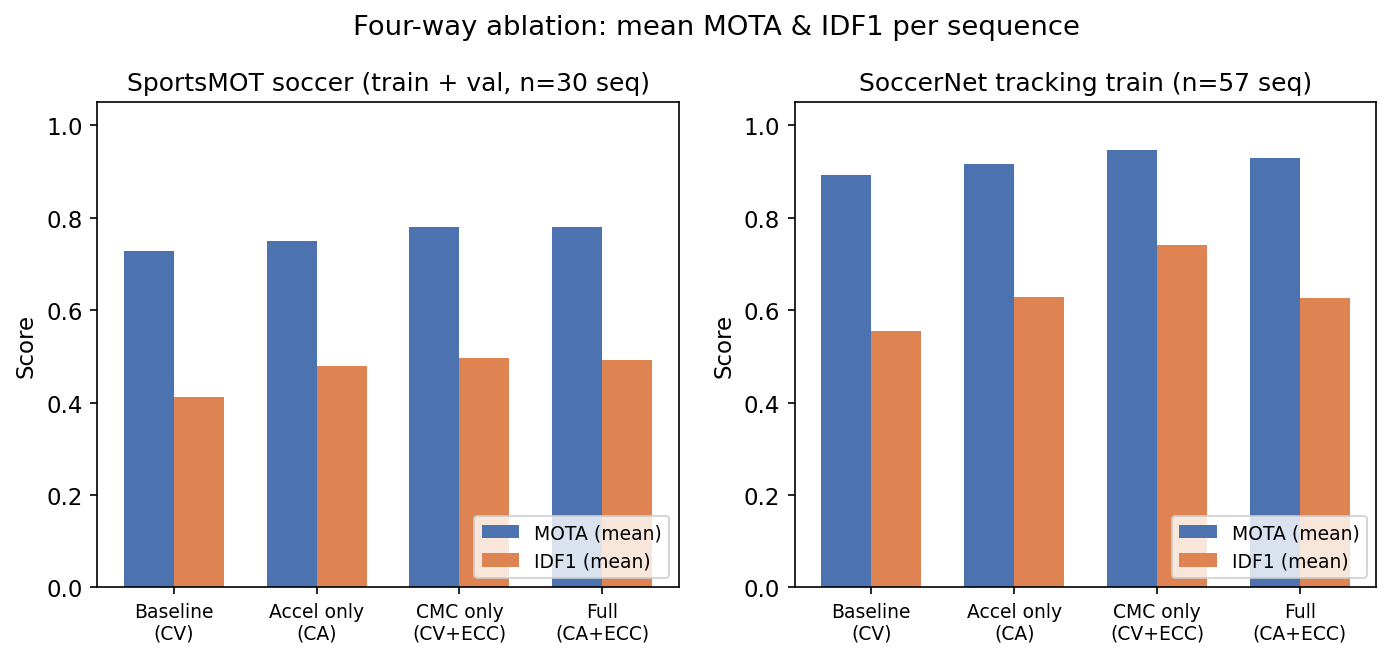
\includegraphics[width=\linewidth]{fig1_ablation_mota_idf1.png}
  \caption{\textbf{Four-way ablation (tracking).}
  Mean MOTA and IDF1 per sequence on SportsMOT soccer (train+val, 30~seq.;
  \emph{left}) and SoccerNet-Tracking train (57~seq.; \emph{right}).
  Error bars show 95\% confidence intervals over sequences.
  ECC improves both metrics on both datasets.
  \textbf{Full} matches \textbf{CMC-only} on SportsMOT but underperforms
  it on SoccerNet train under shared hyperparameters.}
  \label{fig:ablation_tracking}
\end{figure}

\begin{figure}[t]
  \centering
  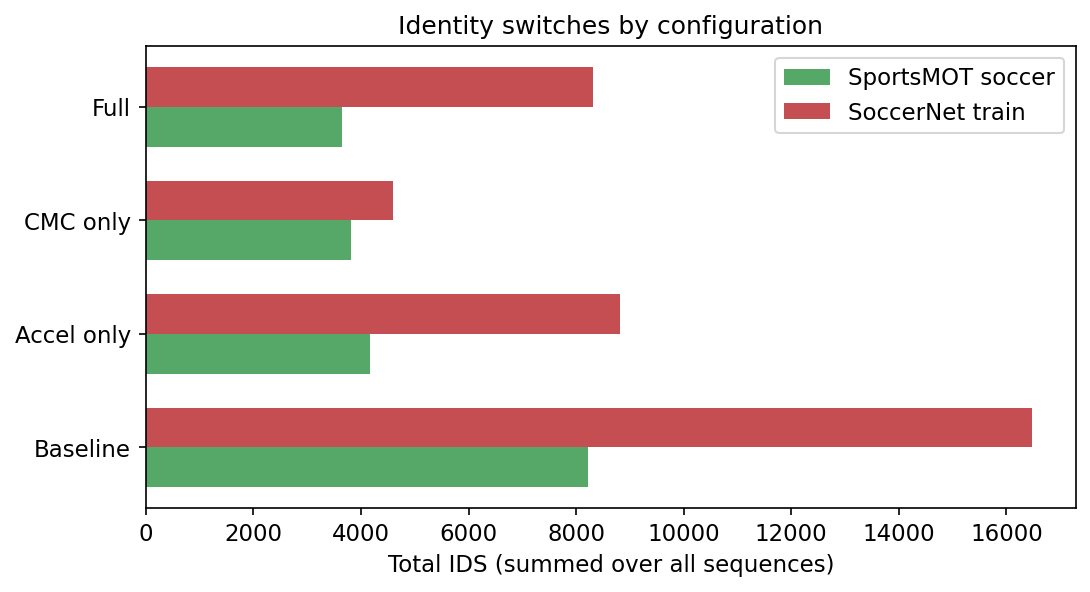
\includegraphics[width=0.92\linewidth]{fig2_ablation_ids_totals.png}
  \caption{\textbf{Identity switches by configuration.}
  Total IDS summed over all sequences (lower is better).
  SportsMOT (\emph{green}) benefits monotonically through \textbf{Full}.
  SoccerNet train (\emph{red}) is best at \textbf{CMC-only};
  \textbf{Full} increases IDS, consistent with lower IDF1 in
  Figure~\ref{fig:ablation_tracking}.}
  \label{fig:ablation_ids}
\end{figure}

\begin{figure}[t]
  \centering
  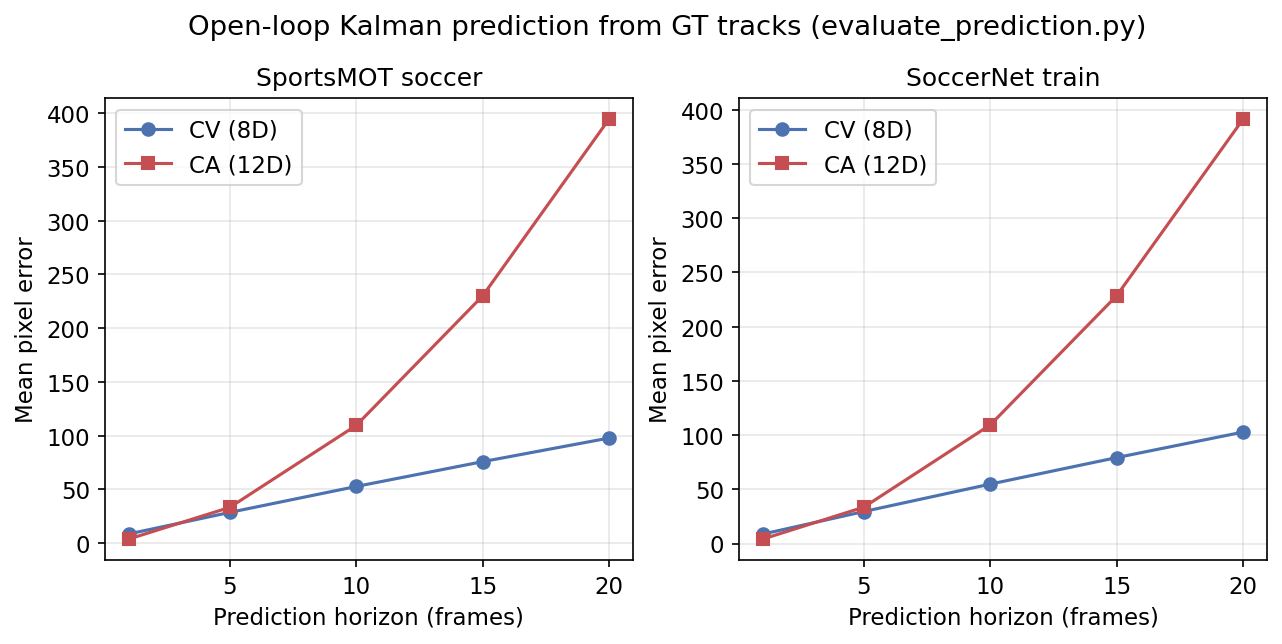
\includegraphics[width=\linewidth]{fig3_prediction_horizon.png}
  \caption{\textbf{Open-loop Kalman prediction error vs.\ horizon.}
  Mean pixel error for CV (8D) vs.\ CA (12D) filters fit to GT tracks on
  SportsMOT soccer (\emph{left}) and SoccerNet train (\emph{right}).
  CA is better at horizon~1 but degrades faster without measurements;
  long-horizon curves should not be equated with tracker association
  performance.}
  \label{fig:prediction_horizon}
\end{figure}

\begin{figure}[t]
  \centering
  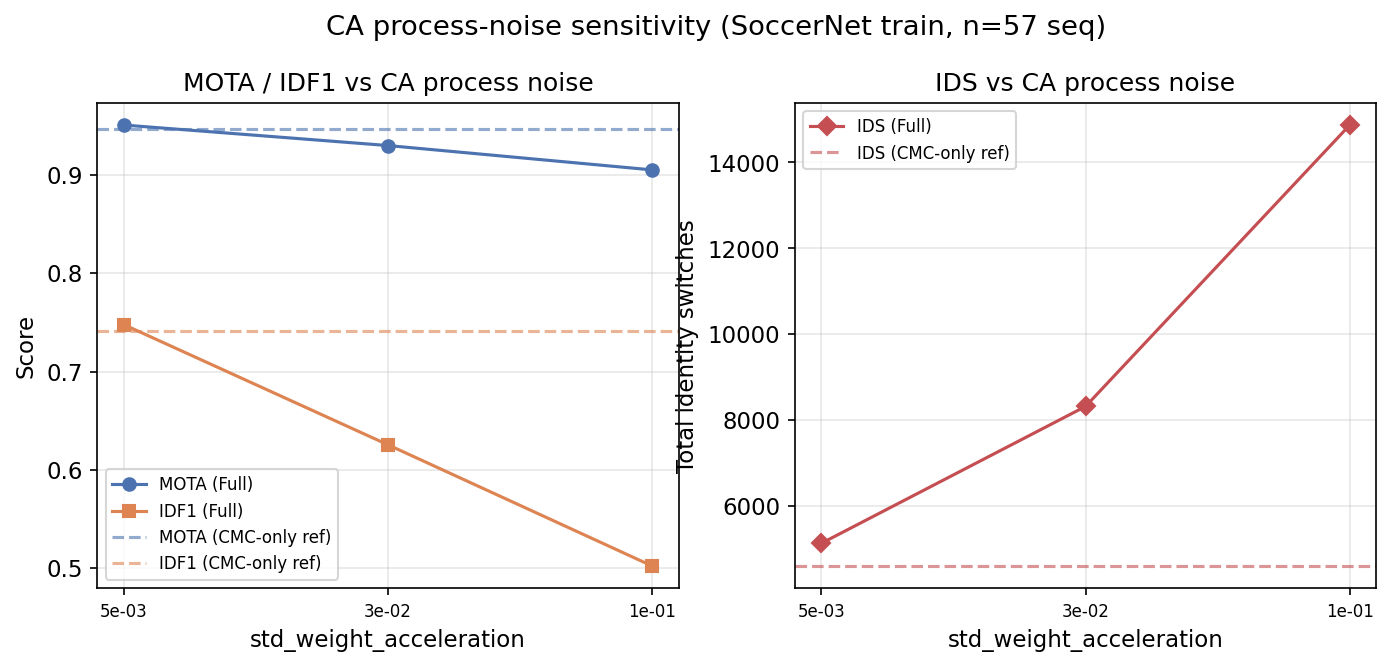
\includegraphics[width=\linewidth]{fig4_ca_sensitivity.png}
  \caption{\textbf{CA process-noise sensitivity (SoccerNet train).}
  MOTA/IDF1 (\emph{left}) and total IDS (\emph{right}) for the Full
  configuration as a function of $\sigma_\mathrm{acc}$. Dashed lines show
  CMC-only reference values. At $\sigma_\mathrm{acc} = 5 \times 10^{-3}$,
  Full matches CMC-only on both metrics; performance degrades monotonically
  with increasing noise, confirming that the main-ablation regression is a
  tuning artifact.}
  \label{fig:ca_sensitivity}
\end{figure}

\begin{figure}[t]
  \centering
  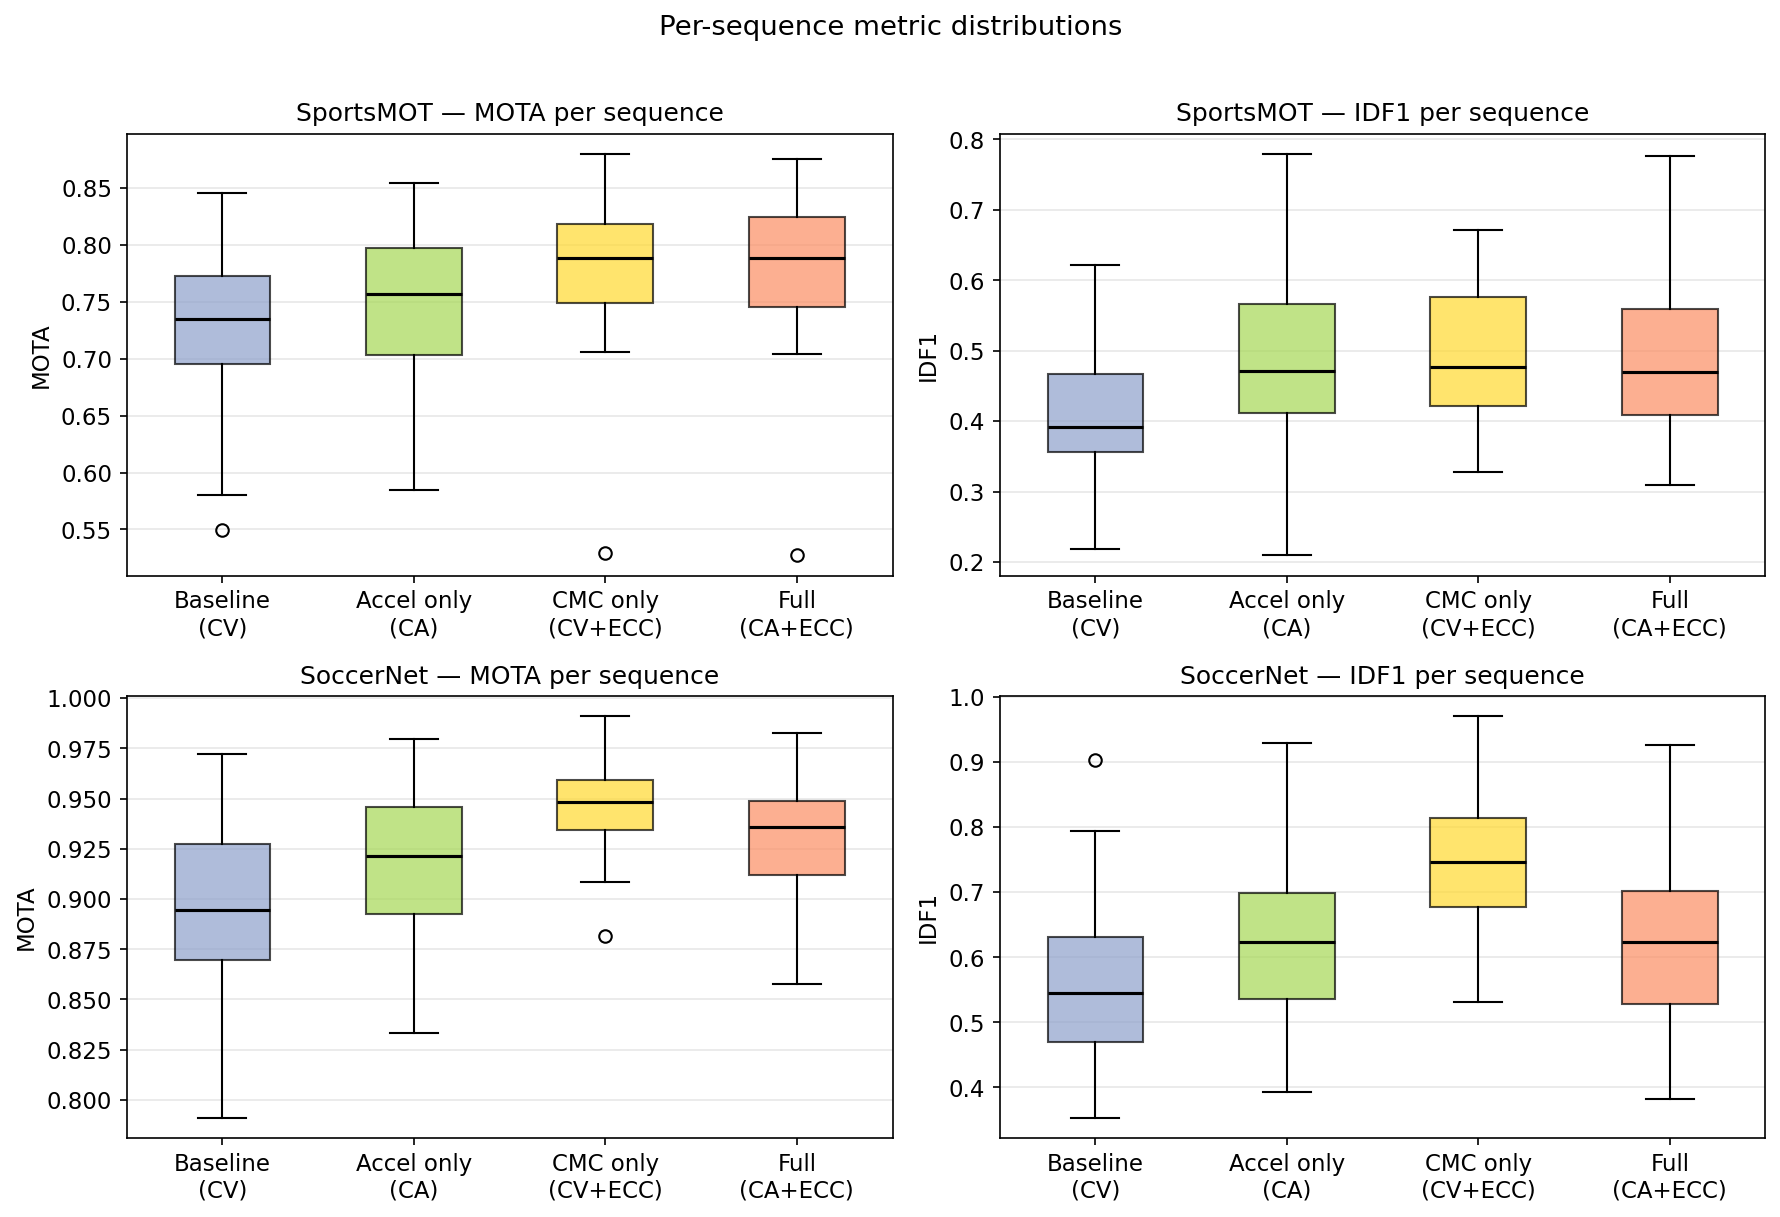
\includegraphics[width=\linewidth]{fig5_per_sequence_boxplots.png}
  \caption{\textbf{Per-sequence metric distributions.}
  Box plots of MOTA (\emph{left}) and IDF1 (\emph{right}) for each
  configuration on SportsMOT (top) and SoccerNet (bottom). On SoccerNet,
  the IDF1 distributions for CMC-only and Full show minimal overlap,
  confirming that the regression is systematic rather than driven by
  outlier sequences.}
  \label{fig:per_sequence_boxplots}
\end{figure}


% =============================================================================
% Tables
% =============================================================================

\begin{table}[t]
  \centering
  \small
  \begin{tabular}{lcccccc}
    \toprule
    & \multicolumn{3}{c}{SportsMOT ($n{=}30$)}
    & \multicolumn{3}{c}{SoccerNet ($n{=}57$)} \\
    \cmidrule(lr){2-4} \cmidrule(lr){5-7}
    Config
    & MOTA$\uparrow$ & IDF1$\uparrow$ & IDS$\downarrow$
    & MOTA$\uparrow$ & IDF1$\uparrow$ & IDS$\downarrow$ \\
    \midrule
    Baseline      & 0.729 & 0.412 & 8228  & 0.893 & 0.556 & 16469 \\
    Accel-only    & 0.749 & 0.480 & 4167  & 0.917 & 0.629 & 8814  \\
    CMC-only      & \textbf{0.781} & \textbf{0.497} & 3808
                  & \textbf{0.947} & \textbf{0.741} & \textbf{4602} \\
    Full          & 0.780 & 0.491 & \textbf{3639}
                  & 0.930 & 0.626 & 8319 \\
    \bottomrule
  \end{tabular}
  \caption{Mean MOTA and IDF1 per sequence; IDS summed over all sequences.
  Best values per dataset in bold. On SportsMOT, Full achieves the lowest
  IDS while matching CMC-only on MOTA/IDF1. On SoccerNet, CMC-only
  dominates across all three metrics.}
  \label{tab:ablation}
\end{table}

\begin{table}[t]
  \centering
  \small
  \begin{tabular}{lcccc}
    \toprule
    & \multicolumn{2}{c}{SportsMOT ($n{=}30$)}
    & \multicolumn{2}{c}{SoccerNet ($n{=}57$)} \\
    \cmidrule(lr){2-3} \cmidrule(lr){4-5}
    Comparison & MOTA & IDF1 & MOTA & IDF1 \\
    \midrule
    Baseline vs.\ Accel-only
      & .001\rlap{$^{**}$}  & $<$.001\rlap{$^{***}$}
      & $<$.001\rlap{$^{***}$} & $<$.001\rlap{$^{***}$} \\
    Baseline vs.\ CMC-only
      & $<$.001\rlap{$^{***}$} & $<$.001\rlap{$^{***}$}
      & $<$.001\rlap{$^{***}$} & $<$.001\rlap{$^{***}$} \\
    Baseline vs.\ Full
      & $<$.001\rlap{$^{***}$} & $<$.001\rlap{$^{***}$}
      & $<$.001\rlap{$^{***}$} & $<$.001\rlap{$^{***}$} \\
    Accel-only vs.\ CMC-only
      & $<$.001\rlap{$^{***}$} & .146\phantom{$^{***}$}
      & $<$.001\rlap{$^{***}$} & $<$.001\rlap{$^{***}$} \\
    Accel-only vs.\ Full
      & $<$.001\rlap{$^{***}$} & .855\phantom{$^{***}$}
      & $<$.001\rlap{$^{***}$} & .015\rlap{$^{*}$}\phantom{$^{**}$} \\
    CMC-only vs.\ Full
      & .253\phantom{$^{***}$} & .029\phantom{$^{***}$}
      & $<$.001\rlap{$^{***}$} & $<$.001\rlap{$^{***}$} \\
    \bottomrule
  \end{tabular}
  \caption{Paired Wilcoxon signed-rank $p$-values (two-sided, uncorrected).
  $^{*}\!p<.05$,\; $^{**}\!p<.01$,\; $^{***}\!p<.001$.
  All configurations differ significantly from Baseline.
  CMC-only vs.\ Full is not significant on SportsMOT (MOTA $p{=}.25$,
  IDF1 $p{=}.029$ --- would not survive Bonferroni correction for 6
  comparisons) but highly significant on SoccerNet ($p < 10^{-9}$).}
  \label{tab:significance}
\end{table}

\begin{table}[t]
  \centering
  \small
  \begin{tabular}{lccccc}
    \toprule
    & \multicolumn{5}{c}{Identity switches by regime} \\
    \cmidrule(lr){2-6}
    Config & Accel & Pan & Both & Neither & Total \\
    \midrule
    \multicolumn{6}{l}{\emph{SportsMOT (train+val, 30 seq.)}} \\
    Baseline      & 3230 & ---  & ---  & 4998 & 8228 \\
    Accel-only    & 1752 & ---  & ---  & 2415 & 4167 \\
    CMC-only      &  423 &  893 &  826 & 1666 & 3808 \\
    Full          &  356 &  895 &  840 & 1548 & 3639 \\
    \midrule
    \multicolumn{6}{l}{\emph{SoccerNet train (57 seq.)}} \\
    Baseline      & 14054 & --- & ---  & 2415 & 16469 \\
    Accel-only    &  7479 & --- & ---  & 1335 &  8814 \\
    CMC-only      &   607 & 557 & 2838 &  600 &  4602 \\
    Full          &   716 & 435 & 6631 &  537 &  8319 \\
    \bottomrule
  \end{tabular}
  \caption{Identity switches broken down by frame regime. ``---'' indicates
  that pan detection is unavailable without CMC enabled. On SoccerNet, Full
  produces 6{,}631 switches during frames with simultaneous acceleration and
  pan events, vs.\ 2{,}838 for CMC-only---the primary source of the Full
  regression.}
  \label{tab:regime}
\end{table}
 set graphics path,
% e.g. from repository root:
%   \graphicspath{{results/analysis/figures/}}
%
% Or copy the PNGs into your paper's ./figures/ and use that folder instead.
% =============================================================================

\section{Experiments}
\label{sec:experiments}

We evaluate through three complementary protocols: a $2 \times 2$ factorial
ablation of tracker configurations, an open-loop Kalman prediction test on
ground-truth tracks, and a per-frame regime analysis that classifies
identity switches by whether they occur during acceleration events, camera
pans, or both.

A $2 \times 2$ factorial design crossing two binary factors, constant-acceleration
Kalman filter (CA) and ECC camera-motion compensation (CMC), yields four
tracker configurations:

\begin{itemize}
    \item \textbf{Baseline} (constant-velocity KF, no CMC),
    \item \textbf{Accel-only} (constant-acceleration KF, no CMC),
    \item \textbf{CMC-only} (constant-velocity KF with ECC), and
    \item \textbf{Full} (constant-acceleration KF with ECC).
\end{itemize}
All four share the same offline detections, the same Re-ID
configuration, and the same association hyperparameters; only the motion
model and compensation module differ. This ensures that any difference in
tracking metrics is attributable to our modifications rather than to
confounding factors.

We measure the open-loop Kalman prediction quality by fitting both
constant-velocity (8D) and constant-acceleration (12D) filters to
ground-truth bounding-box trajectories. At regular intervals (every 5
frames, after at least 10 frames of history), we predict forward
\emph{without any measurement updates} and record the Euclidean distance
between the predicted and true bounding-box centers at horizons
$h \in \{1, 5, 10, 15, 20\}$ frames. This test isolates the motion model's
extrapolation quality from the association step.

We report standard MOTChallenge metrics computed via the
\texttt{py-motmetrics} library with an IoU matching threshold of 0.5. Our
primary metric is IDF1, which directly measures identity preservation over
time and is the most relevant quantity for sports analytics where correct
player identity matters more than detection completeness. We report MOTA for
comparability with prior work, alongside raw identity-switch counts (IDS)
summed over all sequences.

To test whether the two fixes target separable failure modes, we classify
each frame into one of four regimes based on ground-truth trajectories and
ECC warp estimates. A frame is flagged as an \emph{acceleration event} if
any tracked player's velocity changes by more than 15~px/frame$^2$ within a
$\pm 3$-frame window. A frame is flagged as a \emph{camera-pan event} if the
ECC-estimated affine translation magnitude exceeds 5~px. Frames can be
flagged as both, either, or neither. We then count identity switches
occurring within each regime. If the constant-acceleration filter primarily
reduces switches during acceleration events while CMC primarily reduces
switches during pan events, the two modules address orthogonal failure
modes.


Person detections are generated offline using
YOLOv8x~\cite{jocher2023yolov8} pretrained on COCO. We run inference at
1280-pixel resolution with a confidence threshold of~0.3, retaining only
COCO class~0 (person). The resulting bounding boxes are written in
MOTChallenge text format. At tracking time, an additional confidence filter
at~0.5 and non-maximum suppression are applied. Crucially, all four
DeepSORT ablation variants consume the same detection files, so differences
in MOTA, IDF1, and IDS are attributable solely to the tracker.

We deliberately disable the Re-ID appearance branch by using a dummy
feature extractor that returns zero vectors for all detections. DeepSORT's
cascade matching still runs---confirmed tracks are prioritized by recency,
and an IoU-based fallback handles unmatched detections---but the cosine
distance between any two features is constant, so association depends
entirely on Kalman-predicted position and Mahalanobis/IoU gating. This
design choice isolates the effect of our motion-model modifications: with
appearance features active, improvements from the Kalman filter or CMC could
be masked by the Re-ID network independently correcting association errors.
We note that this makes the ablation a harder test of the motion model and
that our reported metrics are conservative relative to what a
soccer-fine-tuned Re-ID network would achieve.

All DeepSORT variants share the same association and lifecycle parameters:
cosine distance threshold~0.3, IoU fallback gate~0.7, appearance gallery
budget of~100 per track, $\text{max\_age} = 30$ frames before track
deletion, and $n_\text{init} = 3$ hits before track confirmation. For the
constant-velocity filter, process-noise weights are
$\sigma_\text{pos} = 10^{-2}$ and $\sigma_\text{vel} = 10^{-5}$ (scaled by
bounding-box height). The constant-acceleration filter uses the same
position and velocity noise, with an acceleration process-noise weight of
$\sigma_\text{acc} = 2.5 \times 10^{-2}$. This deliberately high
acceleration noise is a key tuning decision: it allows the filter to absorb
sudden directional changes---a player cutting left after sprinting
right---without remaining overconfident in a now-stale acceleration
estimate.

Camera-motion compensation uses OpenCV's Enhanced Correlation Coefficient
(ECC) algorithm in affine mode (6~DOF: translation, rotation, scale, shear).
We set the maximum iteration count to~50 with a convergence threshold of
$10^{-3}$. Frames are downscaled by a factor of~2 and Gaussian-blurred with
$\sigma = 1.5$ before ECC estimation, balancing speed against registration
robustness. When ECC fails to converge (e.g., during shot changes), the
identity warp is applied, resulting in no compensation for that frame.


% ─────────────────────────────────────────────────────────────────────────────
\subsection{Results}
\label{sec:results}
% ─────────────────────────────────────────────────────────────────────────────


We evaluate four tracker variants as described in
Section~\ref{sec:experiments}. We report MOTA and IDF1 averaged over
sequences and IDS summed over sequences (fewer identity switches is better).
On the SportsMOT soccer subset we pool the train and validation splits
(30~sequences, 53{,}913~frames); on
SoccerNet-Tracking~\cite{cioppa2022soccernettracking} we evaluate the train
split (57~sequences, 42{,}750~frames). Pooling train and validation on
SportsMOT gives a larger and more stable per-variant comparison on a fixed
set of sequences; readers seeking benchmark-aligned headline numbers may
prefer validation- or test-only evaluation.

SportsMOT sequences ship with per-frame detections; where missing, we
generate person-class boxes with YOLOv8x ($\mathrm{conf} > 0.3$).
SoccerNet-Tracking provides annotation-derived detections with the dataset.
Because detector quality and recall differ, cross-dataset metric comparisons
reflect joint tracker\,+\,detector performance and should be interpreted
accordingly. All within-dataset ablation comparisons use identical
detections and thus isolate tracker contributions.


Table~\ref{tab:ablation} and Figure~\ref{fig:ablation_tracking} show mean
MOTA and IDF1 per sequence for each configuration, with error bars
indicating 95\% confidence intervals computed over sequences.
On \textbf{SportsMOT}, enabling camera compensation
yields the largest gains: CMC-only and Full both reach MOTA~$\approx 0.78$,
clearly above Baseline ($\approx 0.73$). IDF1 follows the same trend, with
CMC-only slightly strongest among the ECC variants. On
\textbf{SoccerNet train}, CMC-only is best overall (MOTA~$\approx 0.95$,
IDF1~$\approx 0.74$). Adding acceleration on top of ECC (Full) does not
improve headline metrics on this split; MOTA and especially IDF1 drop
relative to CMC-only, while Accel-only remains a substantial improvement
over Baseline.

Figure~\ref{fig:ablation_ids} reports the same trend through identity
switches. On SportsMOT, IDS decreases monotonically from Baseline through
Full, confirming that the two fixes are complementary on this dataset. On
SoccerNet, IDS is lowest for CMC-only and rises again for Full.

\paragraph{Statistical significance.}
Paired Wilcoxon signed-rank tests (Table~\ref{tab:significance}) confirm
that every configuration differs significantly from Baseline on both
datasets ($p < .002$, uncorrected). On SportsMOT, the difference between
CMC-only and Full is \emph{not} significant for MOTA ($p = .25$); the
nominal $p = .029$ for IDF1 would not survive Bonferroni correction for the
six pairwise comparisons ($\alpha_\text{adj} = .05/6 \approx .008$),
consistent with the overlapping confidence intervals in
Figure~\ref{fig:ablation_tracking}. On SoccerNet, the CMC-only vs.\ Full
gap is highly significant for both metrics ($p < 10^{-9}$, well below any
corrected threshold), confirming that the regression is systematic rather
than driven by a few outlier sequences. Per-sequence distributions
(Figure~\ref{fig:per_sequence_boxplots}) corroborate this: the SoccerNet
IDF1 boxes for CMC-only and Full show minimal overlap.

Together, Figures~\ref{fig:ablation_tracking}--\ref{fig:ablation_ids}
and Table~\ref{tab:significance} indicate that \textbf{ECC camera-motion
compensation is the dominant improvement under shared hyperparameters}.
Combining the constant-acceleration KF with ECC improves identity stability
on SportsMOT but hurts it on SoccerNet train in our configuration,
suggesting that the acceleration noise parameters require dataset-dependent
tuning rather than a universally optimal ``full'' stack.

\paragraph{Regime analysis.}
To diagnose where the Full configuration fails, we classify each identity
switch by what was happening in that frame (Table~\ref{tab:regime}). On
SportsMOT, moving from Baseline to Accel-only reduces acceleration-regime
IDS from 3{,}230 to 1{,}752 (46\% reduction). CMC-only reduces it further
to~423 (87\% vs.\ Baseline). Full provides marginal additional reduction
(356) with similar pan-regime counts, consistent with the complementary
behavior observed above.

On SoccerNet, the pattern is more revealing. Baseline produces 14{,}054
acceleration-regime IDS; Accel-only cuts this to 7{,}479 (47\%). CMC-only
reduces acceleration-regime IDS to 607 but produces 2{,}838 switches in
frames with simultaneous acceleration and pan events. Full \emph{increases}
this both-regime count to 6{,}631---nearly all of the IDS regression
originates in these complex frames where both player acceleration and camera
motion occur simultaneously.

The divergent behavior between datasets has a plausible explanation.
SportsMOT sequences are short clips (typically under 2{,}000~frames) filmed
from overhead cameras with moderate panning, where bursty player motion is
the primary source of prediction error. SoccerNet sequences are longer
broadcast footage with aggressive panning and zooming, where camera
ego-motion dominates. In the SoccerNet regime, the additional acceleration
states in the 12D filter introduce extra degrees of freedom that, without
dataset-specific noise tuning, can amplify drift during extended occlusions.
This is consistent with the well-known bias--variance tradeoff in Kalman
filter design: a higher-dimensional state improves fit to complex dynamics
but increases estimation noise when measurements are sparse.

\paragraph{Process-noise sensitivity.}
To investigate whether the Full-configuration regression on SoccerNet is
structural or parametric, we sweep the CA process-noise scale
$\sigma_\mathrm{acc} \in \{5 \times 10^{-3},\; 2.5 \times 10^{-2},\;
10^{-1}\}$ with ECC enabled (Figure~\ref{fig:ca_sensitivity}).
At the lowest noise value ($\sigma_\mathrm{acc} = 5 \times 10^{-3}$),
the Full configuration achieves MOTA\,=\,0.951 and IDF1\,=\,0.748,
\emph{matching or slightly exceeding} the CMC-only reference
(MOTA\,=\,0.947, IDF1\,=\,0.741). Performance degrades monotonically
as noise increases: the default value used in the main ablation
($\sigma_\mathrm{acc} = 2.5 \times 10^{-2}$) already falls well below
CMC-only, and at $10^{-1}$ the tracker loses over 14{,}800 identities.
This confirms that the regression is a tuning artifact rather than a
fundamental incompatibility between CA dynamics and ECC-stabilized
coordinates: with conservative acceleration noise, the 12D filter
neither helps nor hurts on SoccerNet, while retaining its benefits on
SportsMOT.

\subsection{Kalman prediction analysis}

Figure~\ref{fig:prediction_horizon} compares the open-loop center error of
the constant-velocity (8D) and constant-acceleration (12D) Kalman filters
fit to ground-truth tracks at prediction horizons
$h \in \{1, 5, 10, 15, 20\}$ frames. On both datasets, the
constant-acceleration filter achieves \textbf{lower error at $h = 1$},
confirming that one-step prediction benefits from modeling acceleration.
However, error grows faster for the CA filter at longer horizons, surpassing
the CV filter by $h \geq 5$.

This behavior is expected when forecasting without measurements: the extra
acceleration state helps capture immediate dynamics but amplifies drift when
no corrective observations are available. We emphasize that
Figure~\ref{fig:prediction_horizon} is \emph{not} contradictory with the
tracker metrics. In the actual tracking loop, measurement updates arrive
every frame, so the Kalman filter rarely operates in open-loop mode for more
than a few frames (except during occlusions). The one-step advantage of the
CA filter is what matters for frame-to-frame association, while the
long-horizon degradation explains why the CA filter can hurt performance
during extended occlusions---precisely the regime where SoccerNet's longer,
more complex sequences expose the weakness.

\subsection{Limitations}

Several limitations apply to our evaluation. First, SportsMOT relies on
generated detections where sequences were missing pre-computed detection
files, while SoccerNet uses its dataset-provided detections. This means the
detection quality is not perfectly controlled across datasets, although it
is controlled within each dataset across all four ablation variants.

Second, we do not report SoccerNet test or challenge splits, as these
require submission to the official evaluation server. Our pooled train+val
evaluation on SportsMOT is kept for stable per-variant comparison rather
than benchmark headline numbers.

Third, our ablation deliberately disables the Re-ID appearance branch to
isolate motion-model effects. Our reported metrics represent a lower bound
on what our modifications would achieve when combined with a
soccer-fine-tuned Re-ID network. Integrating domain-specific appearance
features is a natural extension of this work.

Fourth, all four variants share a single set of hyperparameters. The
SoccerNet results suggest that the constant-acceleration filter's
process-noise covariance would benefit from per-dataset or per-sequence
tuning. Adaptive noise estimation---for example, using innovation-based
scaling~\cite{cao2023observationcentricsortrethinkingsort}---is another
promising direction.


% =============================================================================
% Figures
% =============================================================================

\begin{figure}[t]
  \centering
  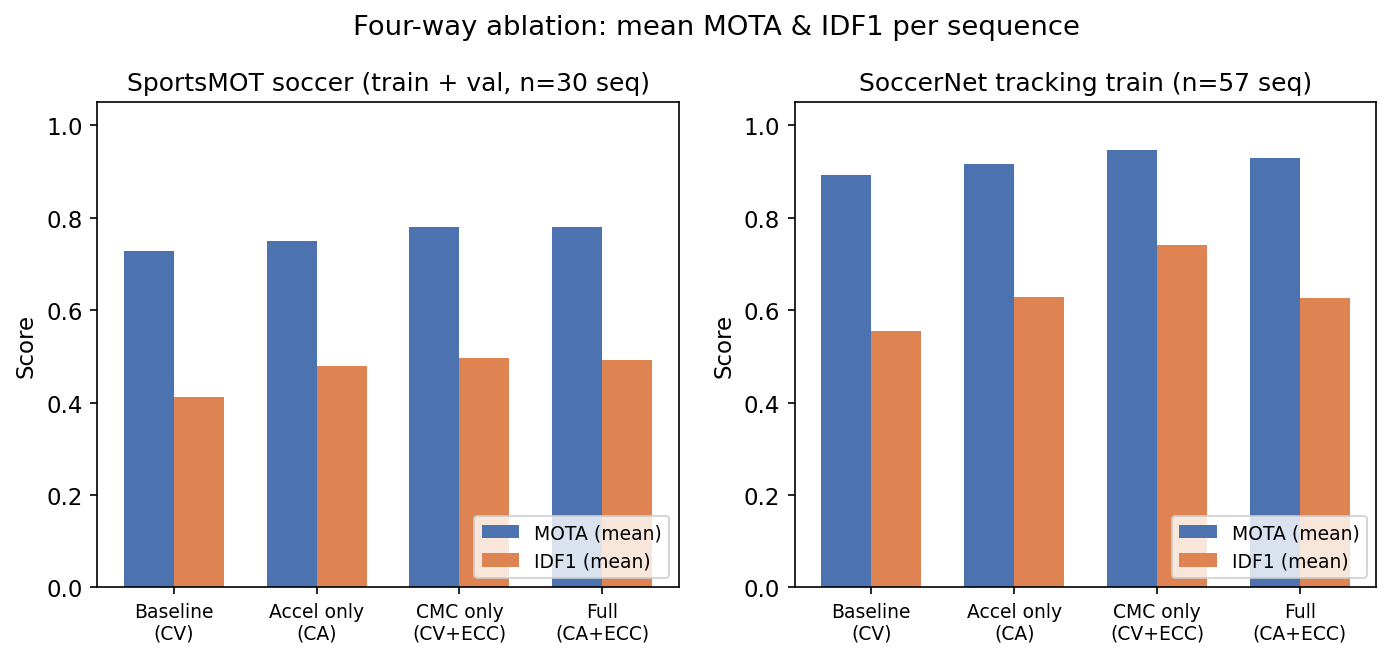
\includegraphics[width=\linewidth]{fig1_ablation_mota_idf1.png}
  \caption{\textbf{Four-way ablation (tracking).}
  Mean MOTA and IDF1 per sequence on SportsMOT soccer (train+val, 30~seq.;
  \emph{left}) and SoccerNet-Tracking train (57~seq.; \emph{right}).
  Error bars show 95\% confidence intervals over sequences.
  ECC improves both metrics on both datasets.
  \textbf{Full} matches \textbf{CMC-only} on SportsMOT but underperforms
  it on SoccerNet train under shared hyperparameters.}
  \label{fig:ablation_tracking}
\end{figure}

\begin{figure}[t]
  \centering
  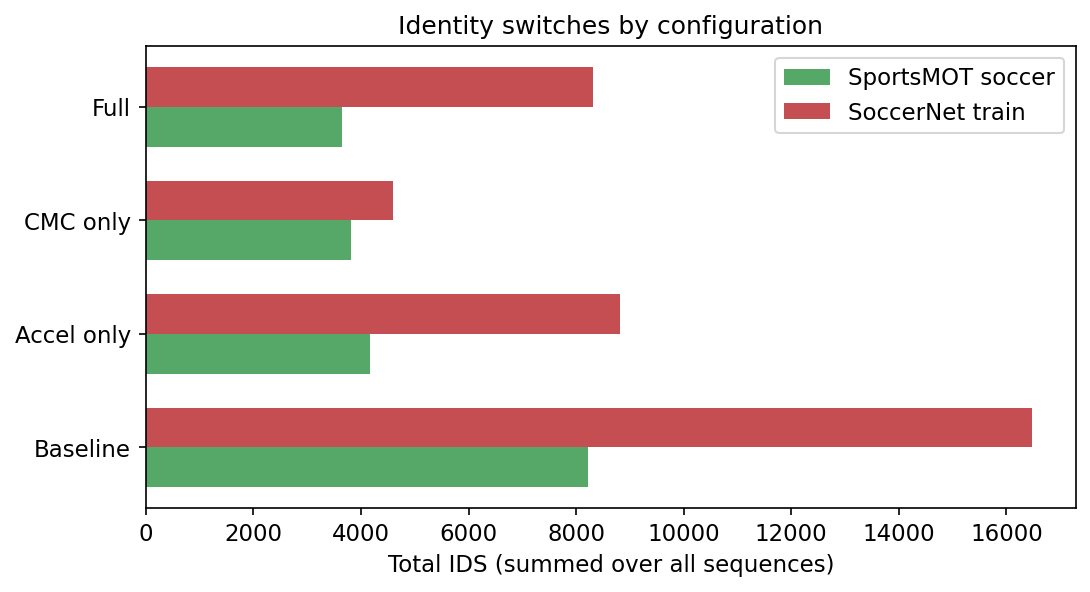
\includegraphics[width=0.92\linewidth]{fig2_ablation_ids_totals.png}
  \caption{\textbf{Identity switches by configuration.}
  Total IDS summed over all sequences (lower is better).
  SportsMOT (\emph{green}) benefits monotonically through \textbf{Full}.
  SoccerNet train (\emph{red}) is best at \textbf{CMC-only};
  \textbf{Full} increases IDS, consistent with lower IDF1 in
  Figure~\ref{fig:ablation_tracking}.}
  \label{fig:ablation_ids}
\end{figure}

\begin{figure}[t]
  \centering
  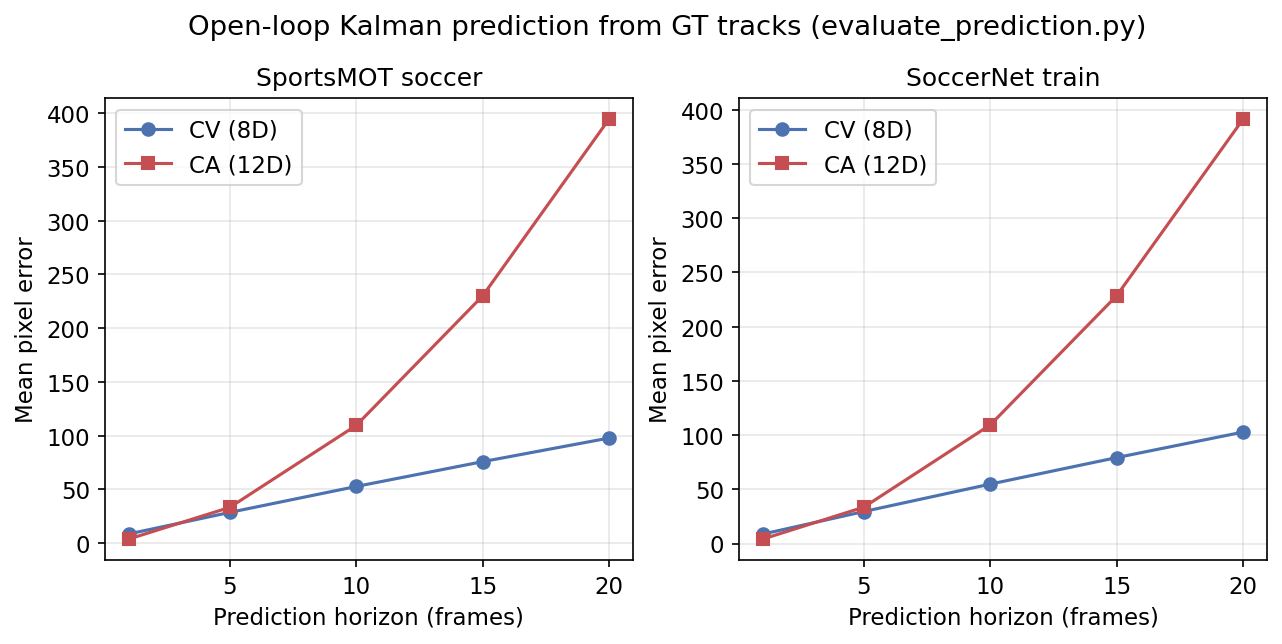
\includegraphics[width=\linewidth]{fig3_prediction_horizon.png}
  \caption{\textbf{Open-loop Kalman prediction error vs.\ horizon.}
  Mean pixel error for CV (8D) vs.\ CA (12D) filters fit to GT tracks on
  SportsMOT soccer (\emph{left}) and SoccerNet train (\emph{right}).
  CA is better at horizon~1 but degrades faster without measurements;
  long-horizon curves should not be equated with tracker association
  performance.}
  \label{fig:prediction_horizon}
\end{figure}

\begin{figure}[t]
  \centering
  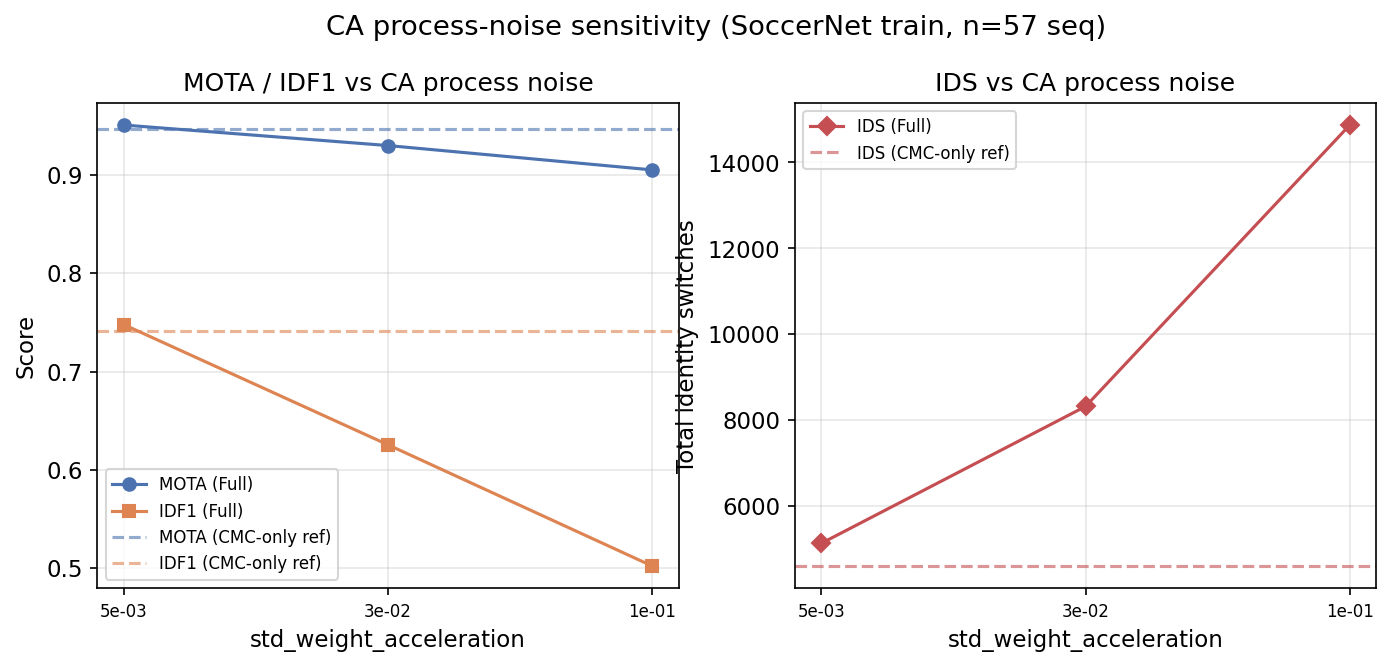
\includegraphics[width=\linewidth]{fig4_ca_sensitivity.png}
  \caption{\textbf{CA process-noise sensitivity (SoccerNet train).}
  MOTA/IDF1 (\emph{left}) and total IDS (\emph{right}) for the Full
  configuration as a function of $\sigma_\mathrm{acc}$. Dashed lines show
  CMC-only reference values. At $\sigma_\mathrm{acc} = 5 \times 10^{-3}$,
  Full matches CMC-only on both metrics; performance degrades monotonically
  with increasing noise, confirming that the main-ablation regression is a
  tuning artifact.}
  \label{fig:ca_sensitivity}
\end{figure}

\begin{figure}[t]
  \centering
  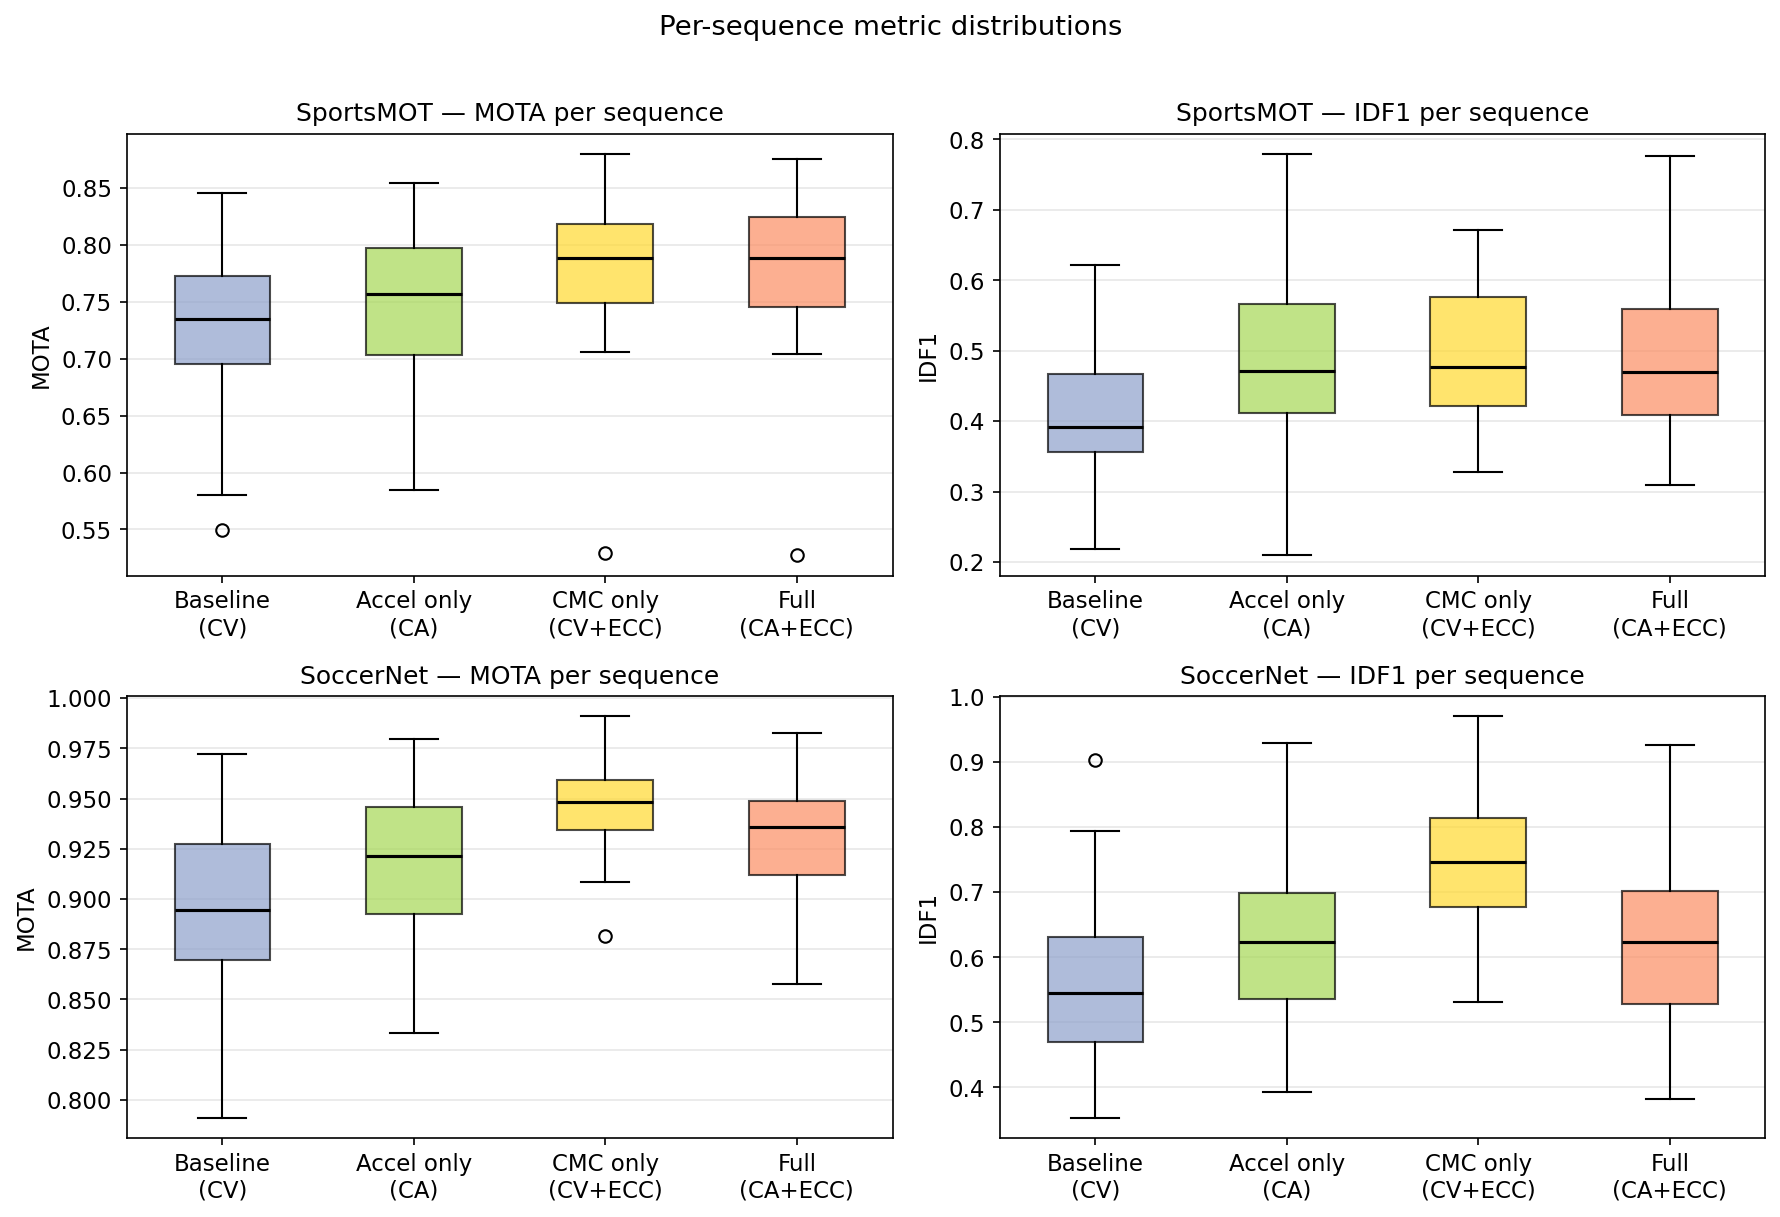
\includegraphics[width=\linewidth]{fig5_per_sequence_boxplots.png}
  \caption{\textbf{Per-sequence metric distributions.}
  Box plots of MOTA (\emph{left}) and IDF1 (\emph{right}) for each
  configuration on SportsMOT (top) and SoccerNet (bottom). On SoccerNet,
  the IDF1 distributions for CMC-only and Full show minimal overlap,
  confirming that the regression is systematic rather than driven by
  outlier sequences.}
  \label{fig:per_sequence_boxplots}
\end{figure}


% =============================================================================
% Tables
% =============================================================================

\begin{table}[t]
  \centering
  \small
  \begin{tabular}{lcccccc}
    \toprule
    & \multicolumn{3}{c}{SportsMOT ($n{=}30$)}
    & \multicolumn{3}{c}{SoccerNet ($n{=}57$)} \\
    \cmidrule(lr){2-4} \cmidrule(lr){5-7}
    Config
    & MOTA$\uparrow$ & IDF1$\uparrow$ & IDS$\downarrow$
    & MOTA$\uparrow$ & IDF1$\uparrow$ & IDS$\downarrow$ \\
    \midrule
    Baseline      & 0.729 & 0.412 & 8228  & 0.893 & 0.556 & 16469 \\
    Accel-only    & 0.749 & 0.480 & 4167  & 0.917 & 0.629 & 8814  \\
    CMC-only      & \textbf{0.781} & \textbf{0.497} & 3808
                  & \textbf{0.947} & \textbf{0.741} & \textbf{4602} \\
    Full          & 0.780 & 0.491 & \textbf{3639}
                  & 0.930 & 0.626 & 8319 \\
    \bottomrule
  \end{tabular}
  \caption{Mean MOTA and IDF1 per sequence; IDS summed over all sequences.
  Best values per dataset in bold. On SportsMOT, Full achieves the lowest
  IDS while matching CMC-only on MOTA/IDF1. On SoccerNet, CMC-only
  dominates across all three metrics.}
  \label{tab:ablation}
\end{table}

\begin{table}[t]
  \centering
  \small
  \begin{tabular}{lcccc}
    \toprule
    & \multicolumn{2}{c}{SportsMOT ($n{=}30$)}
    & \multicolumn{2}{c}{SoccerNet ($n{=}57$)} \\
    \cmidrule(lr){2-3} \cmidrule(lr){4-5}
    Comparison & MOTA & IDF1 & MOTA & IDF1 \\
    \midrule
    Baseline vs.\ Accel-only
      & .001\rlap{$^{**}$}  & $<$.001\rlap{$^{***}$}
      & $<$.001\rlap{$^{***}$} & $<$.001\rlap{$^{***}$} \\
    Baseline vs.\ CMC-only
      & $<$.001\rlap{$^{***}$} & $<$.001\rlap{$^{***}$}
      & $<$.001\rlap{$^{***}$} & $<$.001\rlap{$^{***}$} \\
    Baseline vs.\ Full
      & $<$.001\rlap{$^{***}$} & $<$.001\rlap{$^{***}$}
      & $<$.001\rlap{$^{***}$} & $<$.001\rlap{$^{***}$} \\
    Accel-only vs.\ CMC-only
      & $<$.001\rlap{$^{***}$} & .146\phantom{$^{***}$}
      & $<$.001\rlap{$^{***}$} & $<$.001\rlap{$^{***}$} \\
    Accel-only vs.\ Full
      & $<$.001\rlap{$^{***}$} & .855\phantom{$^{***}$}
      & $<$.001\rlap{$^{***}$} & .015\rlap{$^{*}$}\phantom{$^{**}$} \\
    CMC-only vs.\ Full
      & .253\phantom{$^{***}$} & .029\phantom{$^{***}$}
      & $<$.001\rlap{$^{***}$} & $<$.001\rlap{$^{***}$} \\
    \bottomrule
  \end{tabular}
  \caption{Paired Wilcoxon signed-rank $p$-values (two-sided, uncorrected).
  $^{*}\!p<.05$,\; $^{**}\!p<.01$,\; $^{***}\!p<.001$.
  All configurations differ significantly from Baseline.
  CMC-only vs.\ Full is not significant on SportsMOT (MOTA $p{=}.25$,
  IDF1 $p{=}.029$ --- would not survive Bonferroni correction for 6
  comparisons) but highly significant on SoccerNet ($p < 10^{-9}$).}
  \label{tab:significance}
\end{table}

\begin{table}[t]
  \centering
  \small
  \begin{tabular}{lccccc}
    \toprule
    & \multicolumn{5}{c}{Identity switches by regime} \\
    \cmidrule(lr){2-6}
    Config & Accel & Pan & Both & Neither & Total \\
    \midrule
    \multicolumn{6}{l}{\emph{SportsMOT (train+val, 30 seq.)}} \\
    Baseline      & 3230 & ---  & ---  & 4998 & 8228 \\
    Accel-only    & 1752 & ---  & ---  & 2415 & 4167 \\
    CMC-only      &  423 &  893 &  826 & 1666 & 3808 \\
    Full          &  356 &  895 &  840 & 1548 & 3639 \\
    \midrule
    \multicolumn{6}{l}{\emph{SoccerNet train (57 seq.)}} \\
    Baseline      & 14054 & --- & ---  & 2415 & 16469 \\
    Accel-only    &  7479 & --- & ---  & 1335 &  8814 \\
    CMC-only      &   607 & 557 & 2838 &  600 &  4602 \\
    Full          &   716 & 435 & 6631 &  537 &  8319 \\
    \bottomrule
  \end{tabular}
  \caption{Identity switches broken down by frame regime. ``---'' indicates
  that pan detection is unavailable without CMC enabled. On SoccerNet, Full
  produces 6{,}631 switches during frames with simultaneous acceleration and
  pan events, vs.\ 2{,}838 for CMC-only---the primary source of the Full
  regression.}
  \label{tab:regime}
\end{table}
